\documentclass[12pt,a4paper,twoside,openright]{llncs}

               %%%%%%%%%%%%%%%%%%%%%%%%%%%%%%%%%%%%%%
               %    Scelta dei package da usare     %
               %%%%%%%%%%%%%%%%%%%%%%%%%%%%%%%%%%%%%%

\usepackage[utf8]{inputenc}
%%\usepackage{amsmath,amsfonts,amssymb,amsthm}
\usepackage[english]{babel}
\usepackage[T1]{fontenc}
\usepackage{url}
\usepackage{xspace}
\usepackage{fancyhdr}
\usepackage{graphicx}
\usepackage{eurosym}
\usepackage{afterpage}
\usepackage{float}
\usepackage{wrapfig}
\usepackage{lscape}
\usepackage{rotating}
\usepackage{epstopdf}

\makeatletter

\usepackage{manifest}

\makeatother

               %%%%%%%%%%%%%%%%%%%%%%%%%%%%%%%%%%%%%%%%
               % Scelta delle dimensioni della pagina %
               %%%%%%%%%%%%%%%%%%%%%%%%%%%%%%%%%%%%%%%%

\setlength{\textwidth}{13.5cm}
\setlength{\textheight}{19cm}
\setlength{\footskip}{3cm}
\setlength{\parskip}{0.5em}
\setlength{\parindent}{1em}

               %%%%%%%%%%%%%%%%%%%%%%%%%%%%%%%%%%%%
               %    Reduce Section Spaceing       %
               %%%%%%%%%%%%%%%%%%%%%%%%%%%%%%%%%%%%

%% sudo apt-get install texlive-latex-extra required.


%% Save the class definition of \subparagraph
\let\llncssubparagraph\subparagraph
%% Provide a definition to \subparagraph to keep titlesec happy
\let\subparagraph\paragraph
%% Load titlesec
\usepackage[compact]{titlesec}
%% Revert \subparagraph to the llncs definition
\let\subparagraph\llncssubparagraph

\titlespacing{\section}{0pt}{2ex}{1ex}
\titlespacing{\subsection}{0pt}{1ex}{0ex}
\titlespacing{\subsubsection}{0pt}{0.5ex}{0ex}

               %%%%%%%%%%%%%%%%%%%%%%%%%%%%%%%%%%%%%
               % Commands inseriti per il template %
               %               di Natali           %
               %%%%%%%%%%%%%%%%%%%%%%%%%%%%%%%%%%%%%

\newcommand{\java}{\textsf{Java}}
\newcommand{\contact}{\emph{Contact}}
\newcommand{\corecl}{\texttt{corecl}}
\newcommand{\medcl}{\texttt{medcl}}
\newcommand{\msgcl}{\texttt{msgcl}}
\newcommand{\android}{\texttt{Android}}
\newcommand{\dsl}{\texttt{DSL}}
\newcommand{\jazz}{\texttt{Jazz}}
\newcommand{\rtc}{\texttt{RTC}}
\newcommand{\ide}{\texttt{Contact-ide}}
\newcommand{\xtext}{\texttt{XText}}
\newcommand{\xpand}{\texttt{Xpand}}
\newcommand{\xtend}{\texttt{Xtend}}
\newcommand{\pojo}{\texttt{POJO}}
\newcommand{\junit}{\texttt{JUnit}}

\newcommand{\action}[1]{\texttt{#1}\xspace}
\newcommand{\code}[1]{{\small{\texttt{#1}}}\xspace}
\newcommand{\codescript}[1]{{\scriptsize{\texttt{#1}}}\xspace}

% Cross-referencing
\newcommand{\labelsec}[1]{\label{sec:#1}}
\newcommand{\xs}[1]{\sectionname~\ref{sec:#1}}
\newcommand{\xsp}[1]{\sectionname~\ref{sec:#1} \onpagename~\pageref{sec:#1}}
\newcommand{\labelssec}[1]{\label{ssec:#1}}
\newcommand{\xss}[1]{\subsectionname~\ref{ssec:#1}}
\newcommand{\xssp}[1]{\subsectionname~\ref{ssec:#1} \onpagename~\pageref{ssec:#1}}
\newcommand{\labelsssec}[1]{\label{sssec:#1}}
\newcommand{\xsss}[1]{\subsectionname~\ref{sssec:#1}}
\newcommand{\xsssp}[1]{\subsectionname~\ref{sssec:#1} \onpagename~\pageref{sssec:#1}}
\newcommand{\labelfig}[1]{\label{fig:#1}}
\newcommand{\xf}[1]{\figurename~\ref{fig:#1}}
\newcommand{\xfp}[1]{\figurename~\ref{fig:#1} \onpagename~\pageref{fig:#1}}
\newcommand{\labeltab}[1]{\label{tab:#1}}
\newcommand{\xt}[1]{\tablename~\ref{tab:#1}}
\newcommand{\xtp}[1]{\tablename~\ref{tab:#1} \onpagename~\pageref{tab:#1}}
% Category Names
\newcommand{\sectionname}{Section}
\newcommand{\subsectionname}{Subsection}
\newcommand{\sectionsname}{Sections}
\newcommand{\subsectionsname}{Subsections}
\newcommand{\secname}{\sectionname}
\newcommand{\ssecname}{\subsectionname}
\newcommand{\secsname}{\sectionsname}
\newcommand{\ssecsname}{\subsectionsname}
\newcommand{\onpagename}{on page}

               %%%%%%%%%%%%%%%%%%%%%%%%%%%%%%%%%%%%%%%%
               % Informazioni generali sul dacumento  %
               %    da usare nell'intestazione        %
               %%%%%%%%%%%%%%%%%%%%%%%%%%%%%%%%%%%%%%%%

\newcommand{\xauthA}{Name1 Surename1}
\newcommand{\xauthB}{Name2 Surename2}
\newcommand{\xauthC}{Name3 Surename3}
\newcommand{\xfaculty}{II Faculty of Engineering}
\newcommand{\xunibo}{Alma Mater Studiorum -- University of Bologna}
\newcommand{\xaddrBO}{viale Risorgimento 2}
\newcommand{\xaddrCE}{via Venezia 52}
\newcommand{\xcityBO}{40136 Bologna, Italy}
\newcommand{\xcityCE}{47023 Cesena, Italy}

\setcounter{tocdepth}{3}
\setcounter{secnumdepth}{3}

\begin{document}

%%%%%%%%%%%%%%%%%%%%%%%%%%%%%%%%%%%%%%%%
%  Inserimento della pagina iniziale   %
%%%%%%%%%%%%%%%%%%%%%%%%%%%%%%%%%%%%%%%%

\title{Project Report Template}

%%% \author{\xauthA \and \xauthB}
\author{\xauthA \and \xauthB \and \xauthC}

%
%%%  \xunibo\\\xaddrCE, \xcityCE\\\email{\{nameA.studentA, nameB.studentB\}@studio.unibo.it}
\institute {  \xunibo\\\xaddrCE, \xcityCE\\\email{\{name1.surename1, name2.surename2, name3.surename3\}@mail.com }}

\maketitle

\tableofcontents

\newpage
%%%%%%%%%%%%%%%%%%%%%%%%%%%%%%%%%%%%%%%%%%%
% inclusione dei capitoli e intestazione  %
%%%%%%%%%%%%%%%%%%%%%%%%%%%%%%%%%%%%%%%%%%%

\section{Introduzione}
\labelsec{intro}

Questo è il template di progetto del corso di smart city dell'università di Bologna. Di seguito sar\'a consultabile tutto il processo di analisi del progetto: modelli, problemi riscontrati e soluzioni adottate, interazione con l'ambiente, sensori utilizzati e il loro collegamento \ldots

Per qualsiasi dubbio in merito fare riferimento agli autori.


\section{Vision}
\labelsec{Vision}

Our vision is to reach rapidly the dream of a smart city: with an environment full of augmentend reality and capable to comunicate directly to the user, take decision and made actions in order to deal expecially with crysis or simply to facilitate the life of every day.

We want expecially to be ready in design and build systems embedded in this context and fullfill the gap between hardware and software because recently the hardware had an exponential grow in term of sensors, elaboration capacity and availability of resources due to the decrease of the hardware itserf.

If also you share the same vision

You are in the right plate.


\section{Obbiettivi}
\labelsec{Goals}

Lo scopo del progetto è quello di implementare concretamente un'applicazione di domotica. Affrontando quindi tutte le problematiche ad essa annesse e fornire una possibile soluzione a queste. Ci auguriamo che questa possa essere di spunto per applicazioni simili e che possa quindi favorirne lo sviluppo.

Sfruttando questo progetto, vogliamo esplorare e apprendere la teoria e i concetti affrontati nel corso di smart city. Quindi tutti gli aspetti riguardanti la gestione di sensori e input provenienti dall'ambiente esterno. Uscendo dalla, tipica, zona di confort classica dei sistemi software.


\newpage




\section{Requisiti}
\labelsec{Requirements}

Si vuole monitorare lo stato ambientale di una stanza. In particolare si vogliono monitorare lo stato di: luce, temperatura, umidit\`a, gas e movimento, mantenendo la possibilit\`a di aggiungere altre tipologie di sensori.

Il sistema dovr\`a dare all'utente la possibilit\`a di inserire, attraverso un'interfaccia web, per ogni tipologia di dato, un'apposito range che indichi i valori ammessi all'interno della stanza in modo che, in caso uno dei valori misurati non risulti conforme alle specifiche, venga indicata una notifica di allarme sull'interfaccia stessa. Questo con l'idea di simulare la possibilit\`a di eseguire delle azioni collegate all'allarme (ad esempio, accensione delle luci o del riscaldamento)

L'utente potr\`a inoltre visualizzare all'interno del sito i valori misurati in tempo reale e il valore dei vari sensori nel tempo.

\subsection{Requisiti Non Funzionali}

Aggiungiamo nei requsiti non funzionali tutte le propriet\`a che il sistema deve avere e che non sono state ufficialmente formalizzate.

\begin{itemize}
  \item Separazione dei compiti e indipendenza tra le parti: garantire i principi SOLID dove \`e possibile evitare che un qualsiasi componente sia strettamente legato ad un'altro.
  \item Reattivit\`a: si visualizzi il Reactive Manifesto per i dettagli delle propriet\`a.
\end{itemize}


\section{Acquisto Hardware}
\labelsec{Hardware Procurement}

Sfortunatamente il primo probelma che si e' incontrato in un progetto come il seguente e' stato la necessita' di acquistare la parte hardware del sistema che si andra' a costruire. Di consequenza si e' messo in atto un processo di ricerca dei sensori, cavi e quant'altro per riuscire a soddisfare i requisiti

\subsection{Dispositivi di Computazione}

Prima di tutto necessitiamo di un dispositivo in grado di computare i dati emessi dai vari sensori e che sia interamente programmabile. Nel corso abbiamo visto due possibilita' che hanno avuto molto successo recentemente:

\begin{itemize}
  \item Arduino
  \item Raspberry Pi
\end{itemize}

Noi abbiamo scelto la seconda opzione perche' abbiamo piu' familiarita' con il dispositivo e perche' risulta piu' facile il riutilizzo dello stesso una volta terminato questo progetto.

Costo del dispositivo: 44,50 \euro

\subsection{Sensori}

Un'altra cosa fondamentale riguarda i sensori necessari per catturare i parametri richiesti. Abbiamo Quindi scelto i sequenti sensori

\begin{table}[]
\centering
\begin{tabular}{lll}
\cline{1-1}
\multicolumn{1}{|c|}{\textbf{Parametri Ambientali}} & \multicolumn{1}{c}{\textbf{Sensori}} & \multicolumn{1}{c}{\textbf{Costo}} \\ \cline{1-1}
Temperatura                               &                                     &                                   \\
Luce                                      &                                     &                                   \\
Movimento                                 &                                     &                                  
\end{tabular}
\caption{Sensor Table}
\label{Sensor Table}
\end{table}

\subsection{Hardware Aggiuntivo}

\begin{table}[]
\centering
\begin{tabular}{lll}
\multicolumn{1}{c}{\textbf{Hardware}} &  & \multicolumn{1}{c}{\textbf{Costo}} \\
Breadboard                            &  &                                   \\
Wires                                 &  &                                   \\
Resistors                             &  &                                  
\end{tabular}
\caption{Addictional Hardware}
\label{Addictional Hardware}
\end{table}

\newpage


\section{Analisi dei Requisiti}
\labelsec{ReqAnalysis}
%===========================================================================
\subsection{Casi D'Uso}
\labelssec{UseCases}

\begin{figure}[ht]
\centering
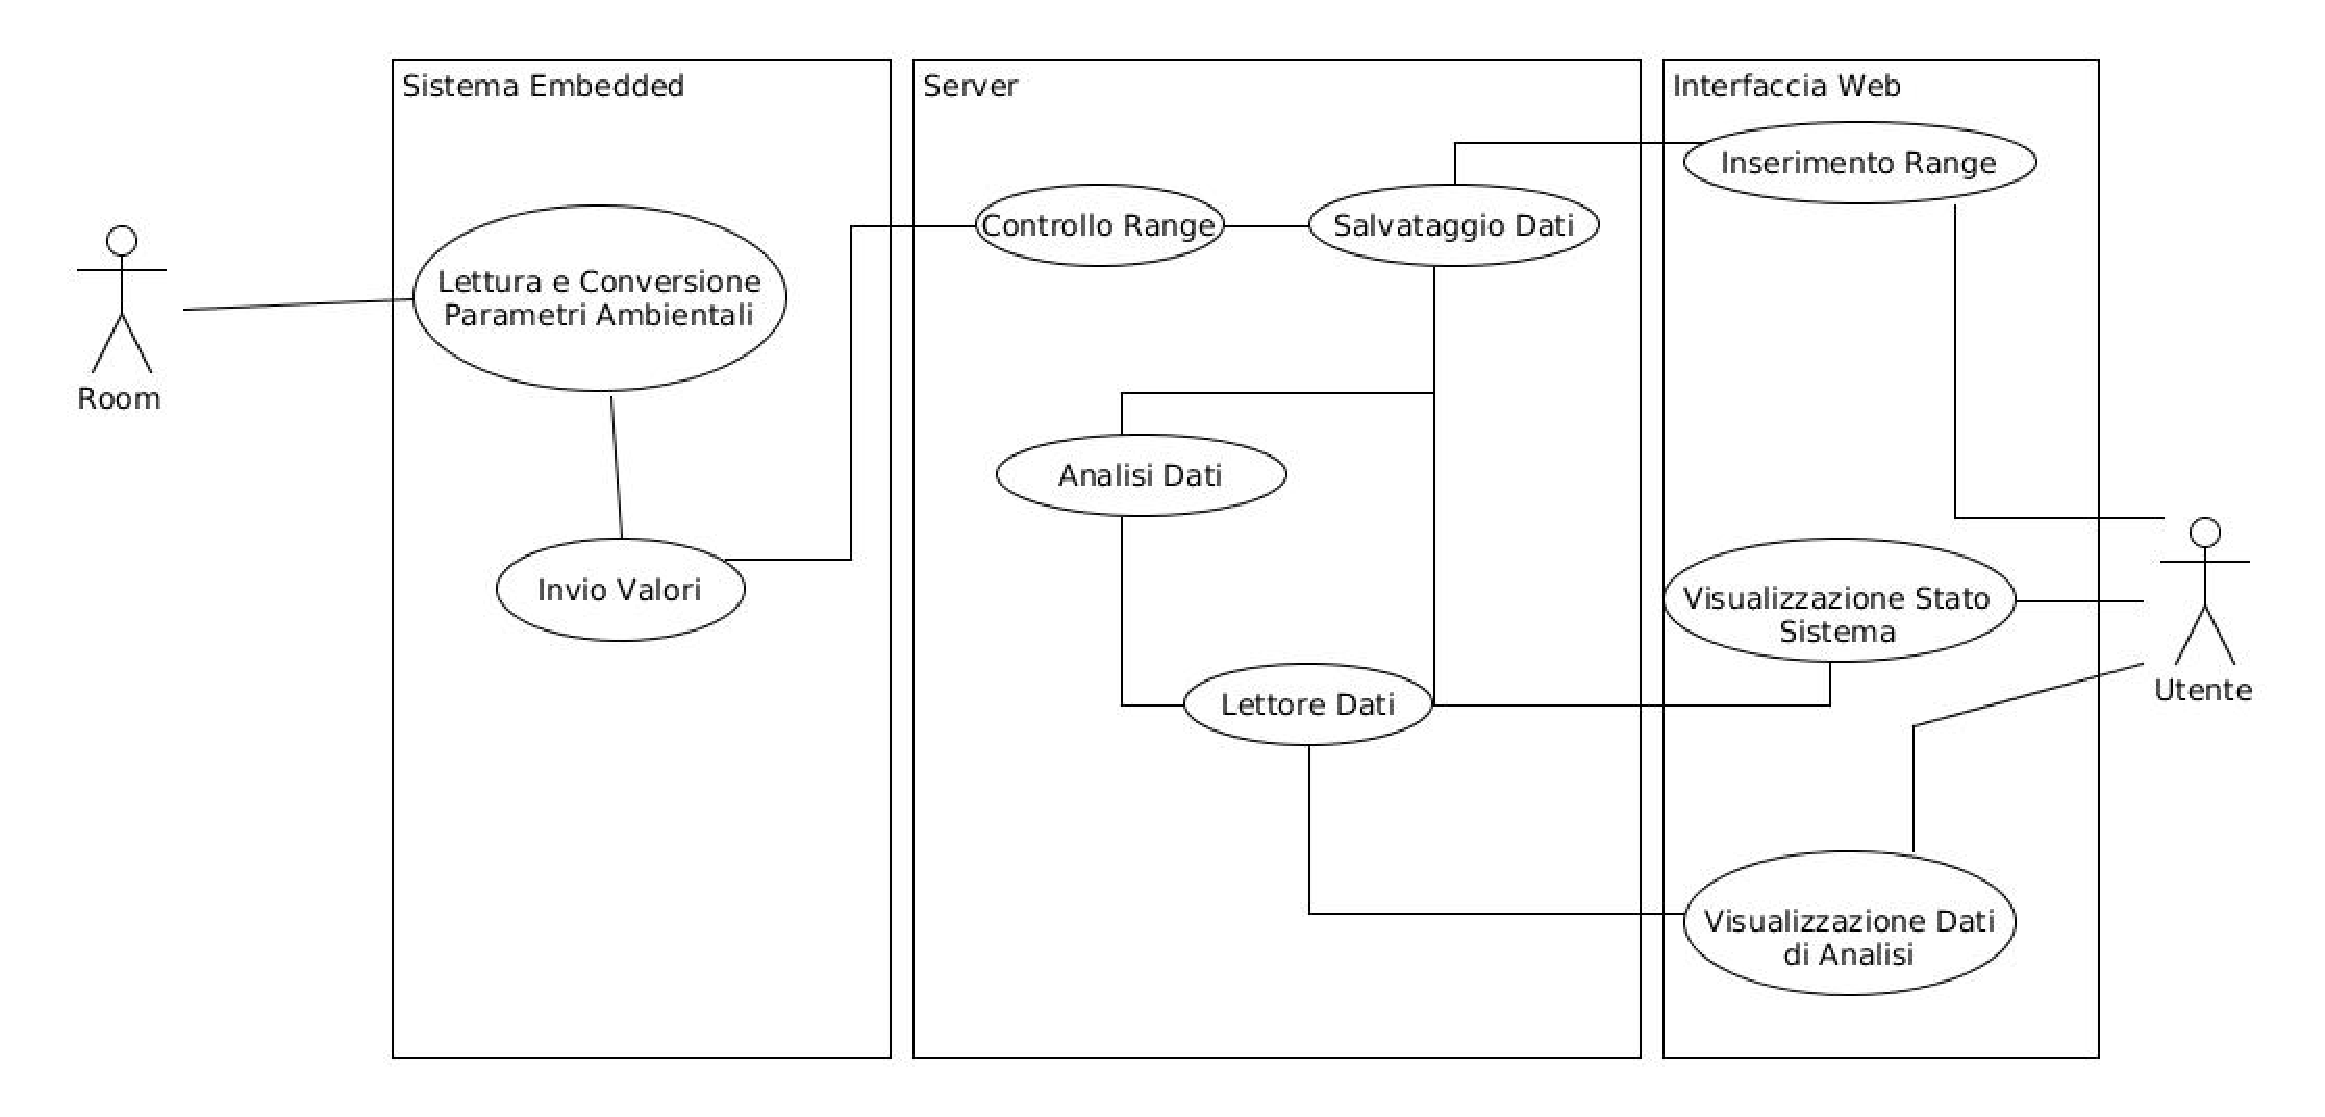
\includegraphics[width=\textwidth]{Figures/UseCases}
\caption{Casi d'Uso}
\end{figure}

Nell'immagine sopra si possono vedere le macro operazioni principali effettuate dal sistema e le interazioni con l'esterno. In particolare gli attori che interagiscono con il sistema saranno:

\begin{itemize}
  \item La stanza: con questo attore si intendono i vari parametri che si possono rilevare attraverso i sensori e che quindi saranno di input per il sistema.
  \item Utente: con questo attore rappresenta l'utente che pu\'o interagire con il sistema.
\end{itemize}

Il sistema \'e stato volutamente suddiviso in tre parti distinte con l'idea di seguire un modello MVC dove la parte di modello non viene aggiornata solamente attraverso l'input inserito dall'utente, ma anche e soprattutto dall'input dei sensori. L'organizzazione hardware ha fortemente influito su questa suddivisione.

\'E inoltre possibile visualizzare le macro operazioni effettuate e modellate dal sistema. Si vedano gli scenari di seguito per avere una pi\'u dettagliata visualizzazione dell'interazione tra le varie parti che lo schema sovrastante vuole rappresentare.


\subsection{Scenario}
\labelssec{Scenarios}

In questa sezione verranno illustrati le principali modalit\'a di utilizzo del sistema. Gli scenari elencati di seguito riguardano l'utente e di conseguenza si prevede l'accesso da parte di questo all'interfaccia di input.

Si prevede che il sistema sia opportunamente configurato e settato a livello hardware, senza errori durante la fase di start up.

\subsubsection{Inserimento Range}

\begin{enumerate}
  \item Attraverso un apposito form l'utente \'e in grado di accedere alla funzionalit\'a di settaggio dei range associati ai parametri ambientali.
  \item Il server conosce gi\'a i sensori collegati al raspberry. Appena questi inviano qualche dato l'utente \'e in grado di visualizzare i controlli relativi ad ogni tipologia di sensore attualmente connesso. Conseguentemente l'utente \'e in grado di modificare tali intervalli.
  \item Al termine della modifica degli intervalli l'utente dovr\'a confermare le modifiche attraverso un'apposito pulsante.
  \item Il sistema mostra un messaggio di conferma o di errore.
\end{enumerate}

\subsubsection{Visualizzazione Stato Realtime}

\paragraph{} All'accesso del sistema l'utente visualizza lo stato realtime dei valori dei sensori ed eventuali notifiche:
\begin{itemize}
  \item Se i valori vanno oltre gli intervalli correnti.
  \item Sullo stato dei sensori, se sono o meno attivi al momento.
\end{itemize}

In questa modalit\'a l'utente non pu\'o effettuare alcuna operazione.

\subsubsection{Visualizzazione Dati}

\paragraph{} Attraverso un apposito men\'u l'utente \'e in grado di accedere alla visualizzazione dei dati storici dei vari sensori.

\newpage

\subsection{Modello del Dominio}

In questa sezione vogliamo cercare di modellare le entit\'a inserite all'interno dei requisiti senza fare riferimento alla parti tecnologiche e hardware. In questo modo siamo in grado di decidere le interfaccie con cui vogliamo lavorare, costruendo la parte software, aumentando il disaccoppiamento con la parte fisica, aumentando anche la possibilit\'a di utilizzare volendo lo stesso software su diverse configurazioni. In questo progetto, ad ogni modo, si utilizzer\'a solamente la configurazione descritta in questo report.

\paragraph{Suddivisione del Sistema:} visto che \'e emerso gi\'a dai casi d'uso la separazione del sistema in varie parti, ci \'e sembrato giusto iniziare a modellare dividendolo fin da subito in modo da:
\begin{itemize}
  \item semplificare il processo
  \item suddividere il lavoro di implementazione successivamente tra i membri del gruppo.
\end{itemize}

In particolare le parti individuate sono tre:

\begin{itemize}
  \item Sistema Embedded: che nel nostro caso si occuper\'a di catturare, convertire e inviare i dati alle altre parti
  \item Server: Sar\'a la parte che riceve i dati e si occupa di effettuare le varie elaborazioni come ad esempio, il salvataggio dei dati, il calcolo delle statistiche e il controllo dei range. Infine questa parte dovr\'a rendere disponibili i risultati alla parte successiva.
  \item Web site: parte che, prendendo i risultati dalle parti precedenti, li mostra all'utente rispettando i casi d'uso predecenti.
\end{itemize}

Chiaramente in questa fase tutto viene semplificato e ridotto a poche entit\'a. Questo per\'o non significa che, ogni entit\'a presente negli schemi sottostanti, non si riveli essere poi a sua volta un sottosistema pi\'u complesso. A sua volta in futuro puo\' accadere di accorpare altre parti insieme. Di conseguenza si vuole mostrare il processo mentale effettuato in ogni fase.

Lo scopo di questa fase \'e appunto quella riflettere, in un primo modello, i requisiti. Successivamente, iniziare a sviluppare il progetto cercando di mantenere coerenza nelle interfaccie principali che indicano le interazioni pi\'u importanti.

\newpage

\subsubsection{Sistema Embedded}

\paragraph{}Per quanto riguarda il sistema embedded \'e necessario prima effettuare delle indagini su come interagire e comunicare con i sensori in modo da modellare adeguatamente il tutto e quindi assicurarsi che in seguito sar\'a semplice riuscire a integrare il tutto con la tecnologia che avremo intenzione di utilizzare. Questa \'e una piccola eccezione che \'e necessario fare a questo livello. Tuttavia si fa riferimento a un paradigma pi\'u che ad una tecnologia specifica.

Data la nostra esperienza del corso e da vari esperimenti intendiamo l'interrogazione del \textbf{il modello di interrogazione dei sensori \'e a polling} di consequenza il nostro modello dovr\'a riflettere questa modalit\'a di interazione. Sfortunatamente questo implica che a livello di modello gi\'a \textbf{un'entit\'a attiva} che si occupa di reperire i valori visto, che in una modalit\'a a polling devo esplicitamente chiedere ai sensori i valori.

\begin{center}
 \textbf{Struttura}
\end{center}

\begin{figure}[h]
\centering
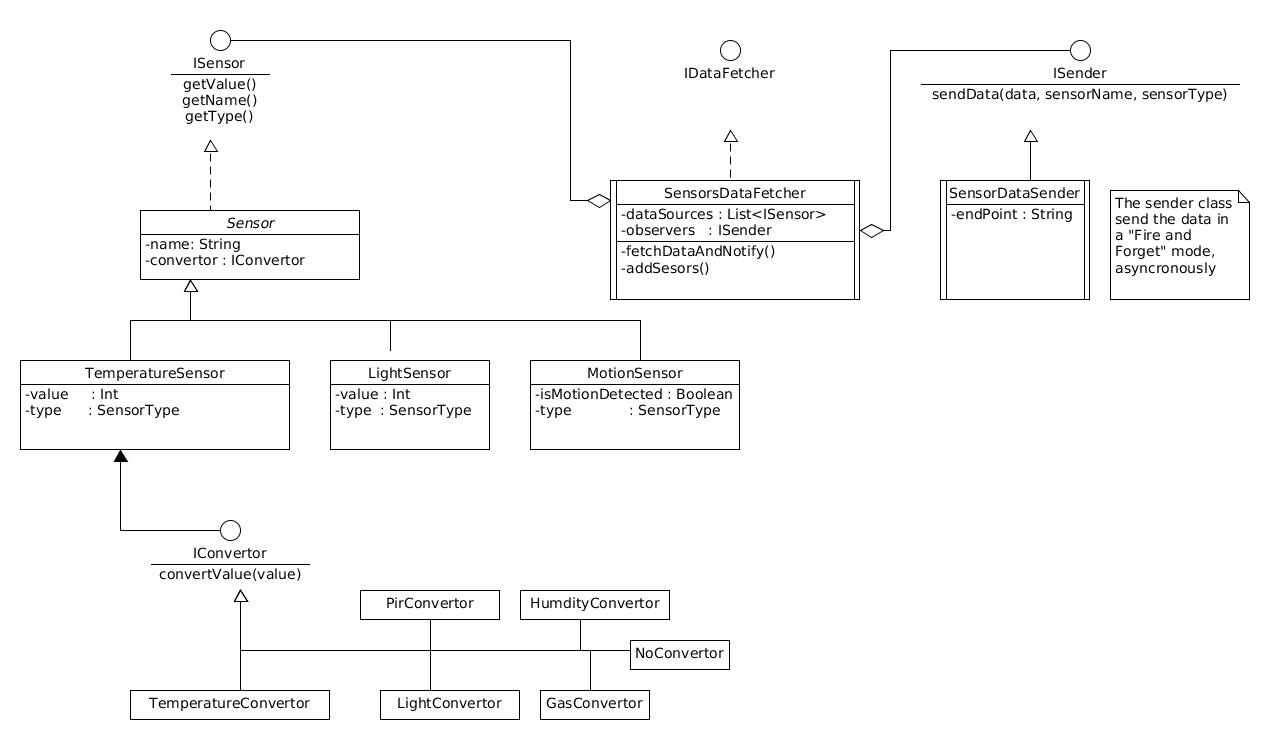
\includegraphics[width=\textwidth]{Figures/DomainModel/EmbeddedSystem/Structure}
\caption{Sistema Embedded, Struttura}
\end{figure}

Dalla struttura \'e possibile individuare subito le entit\'a principali presenti nei requisiti. In particolare la presenza di una specifica gerarchia per i sensori che condividono la stessa interfaccia che consente agilmente di ottenere il valore corrente del sensore. Sono stati inseriti solamente i sensori citati nei requisiti, ma si pu\'o facilmente intuire come qualsiasi tipo di sensore sia facilmente modellabile secondo questa struttura.

Si noti inoltre come viene anche inserita l'entit\'a IConvertor che si occoper\'a di convertire il valore di uno specifico sensore in un'unit\'a pi\'u consona per la sua gestione. Chiaramente questo viene affrontato fin da questo livello perch\'e si immagina l'operazione di conversione come un'operazione quasi istantanea e necessaria.

Infine sono presenti le entit\'a che si occupano, attivamente, di interrogare i sensori ogni intervallo di tempo predefinito e quindi di inviarli altrove. In questo caso \'e stato tutto ridotto ad un singolo endpoint, anche se poi possono essere facilmente pi\'u di uno. Come si pu\'o visionare nel commento, l'invio dei dati avviene con una metodologia di tipo \textit{fire and forget}, quindi non avvengono reinvii dei dati e vengono ignorati eventuali errori. Chiaramente tutto questo \'e dovuto all'idea che i cicli di invio siano abbastanza brevi da potersi permettere eventuali perdite.

\begin{center}
\textbf{Interazione}
\end{center}

Prima di iniziare si vuole evidenziare come viene riportato solamente un diagramma di interazione perch\'e \'e presente solamente un'entit\'a attiva. Tuttavia nel futuro potrebbero esserci pi\'u task e potranno essere necessari pi\'u diagrammi dell'interazione.

Nello schema di interazione vengono evidenziate le varie fasi del Sistema, in particolare la fase iniziale di setup, dove, conoscendo quali sensori sono presenti, questi vengono aggiunti nella memoria dell'entit\'a principale in modo che in seguito siano facilmente interrogabili.

Terminata la fase di \textit{Init} inizia il loop infinito che aspetta inizialmente un piccolo lasso di tempo per poi interrogare iterativamente tutti i sensori che sono stati aggiunti precedentemente, raccogliendo i dati e interrogando asincronamente l'entit\'a di invio, per poi ricominciare il ciclo stesso.

\begin{figure}[h]
\centering
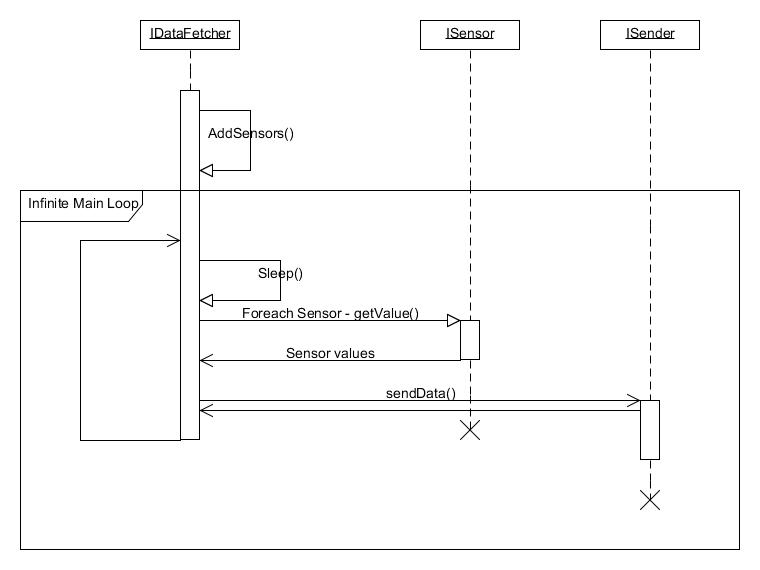
\includegraphics[scale=0.4]{Figures/DomainModel/EmbeddedSystem/Interaction}
\caption{Sistema Embedded, Interazione}
\end{figure}

\newpage

\begin{center}
\textbf{Comportamento}
\end{center}

\begin{figure}[h]
\centering
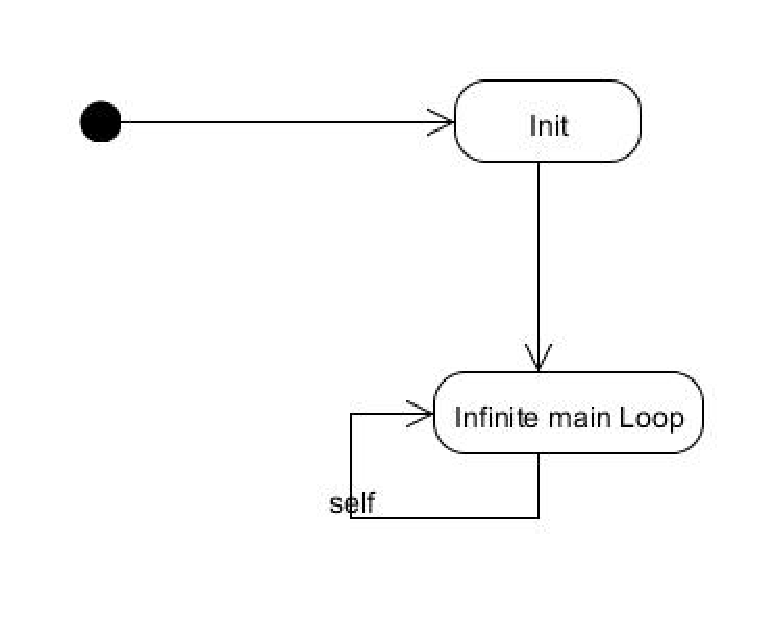
\includegraphics[scale=0.5]{Figures/DomainModel/EmbeddedSystem/Behaviour}
\caption{Sistema Embedded, Comportamento}
\end{figure}


Nel diagramma del comportamento viene semplicemente riportato quanto \'e stato precedentemente discusso attraverso una state machine.

\newpage

\subsubsection{Server}

\paragraph{}La parte server \'e quella pi\'u importante di tutto il sistema in quanto \'e quella che concentra tutta la logica applicativa del sistema stesso.

\begin{center}
\textbf{Struttura}
\end{center}

Le entit\'a principali di questo schema sono:
\begin{itemize}
  \item IPersistentStore, che si occuper\'a di salvare opportunamente i dati provenienti dai sensori e dall'utente
  \item IDataReceiver, che sar\'a sempre in ascolto per ogni messaggio proveniente dal sistema embedded e quindi notificher\'a opportunamente il sistema ad ogni nuovo arrivo
  \item IPresentator che si occuper\'a di ottenere i dati necessari per le viste da mostrare all'utente nel momento in cui una nuova richiesta verr\'a inoltrata.
\end{itemize}

Chiaramente ognuna di queste entit\'a \'e in parte citata nei casi d'uso.

Si vedano i diagrammi dell'interazione per i dettagli di come avviene la comunicazione di tutte queste entit\'a al fronte di garantire il funzionamento e il soddisfacimento dei requisiti.


\begin{figure}[ph]
\centering
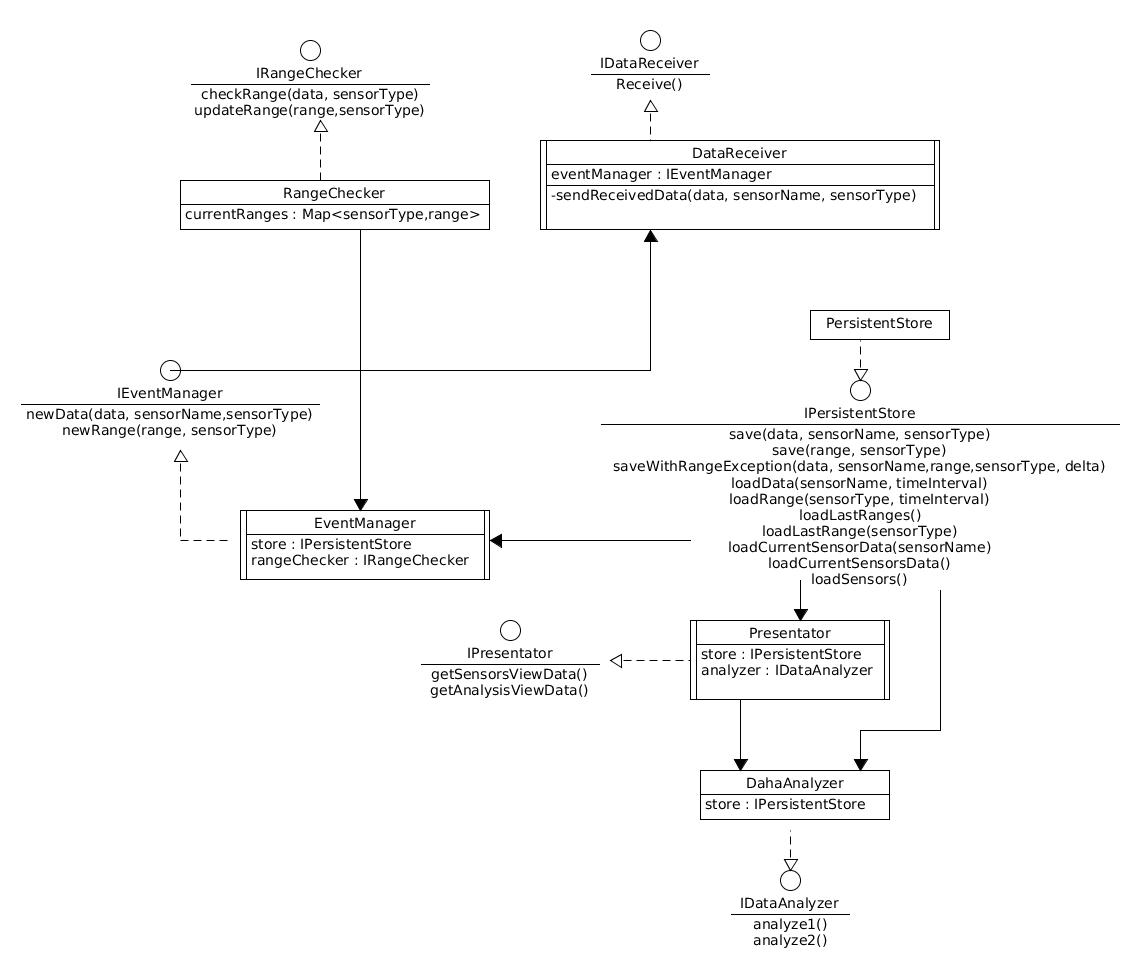
\includegraphics[width=\textwidth,height=\textheight,keepaspectratio]{Figures/DomainModel/Server/Structure}
\caption{Server, Struttura}
\end{figure}

\afterpage{\clearpage}

\newpage

\begin{center}
\textbf{Interazione}
\end{center}

\begin{figure}[h]
\centering
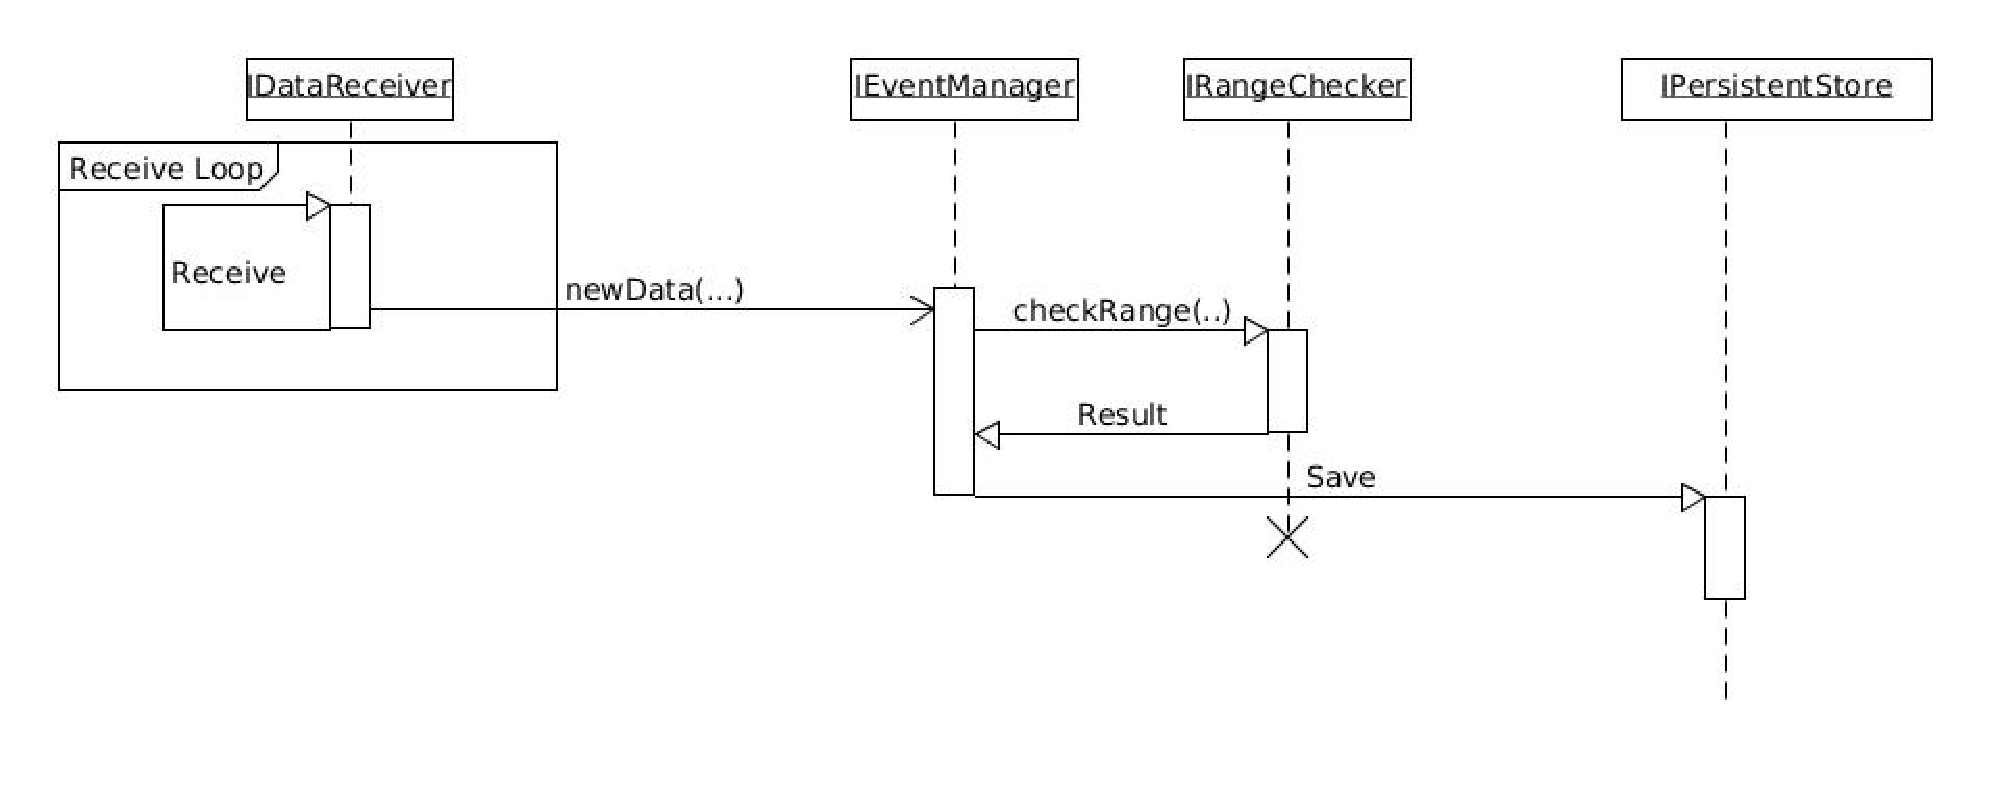
\includegraphics[width=\textwidth]{Figures/DomainModel/Server/NewDataInteraction}
\caption{Server, Interazione, Dati dai Sensori}
\end{figure}

Abbiamo deciso di omettere la parte di inizializzazione del sistema in questa fase dal momento che risulter\'a meglio definita nell'analisi del problema, dovendo aggiungere entit\'a che non sono direttamente correlate con i requisiti principali ma con requisiti non funzionali.

Nello schema sovrastante si pu\'o osservare l'interazione nel caso in cui i sensori emettano un nuovo valore. Si vuole porre particolare enfasi su come l'entit\'a che riceve i dati rimanga sempre in ascolto di nuovi arrivi delegando, tramite una chiamata asincrona alle altre entit\'a, il compito di salvare i dati appena ricevuti.

\newpage

\begin{figure}[h]
\centering
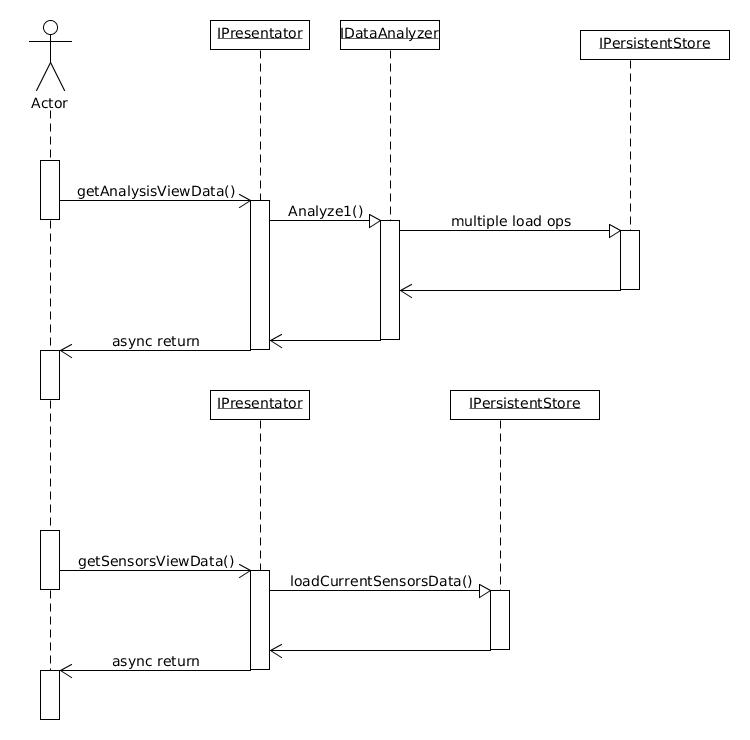
\includegraphics[scale=0.4]{Figures/DomainModel/Server/GetOperationInteraction}
\caption{Server, Interazione, Richiesta Visualizzazione Dati}
\end{figure}

In quest'altro schema dell'interazione si pu\'o osservare che entit\'a vengono coinvolte a fronte di una chiamata di visualizzazione dati da parte dell'utente. Anche in questo caso la chiamata iniziale \'e stata effettuata in maniera asincrona in modo da lasciare il sistema libero di rispondere ad eventuali altre richieste per poterle gestire in mniera concorrente.

\newpage

\begin{figure}[h]
\centering
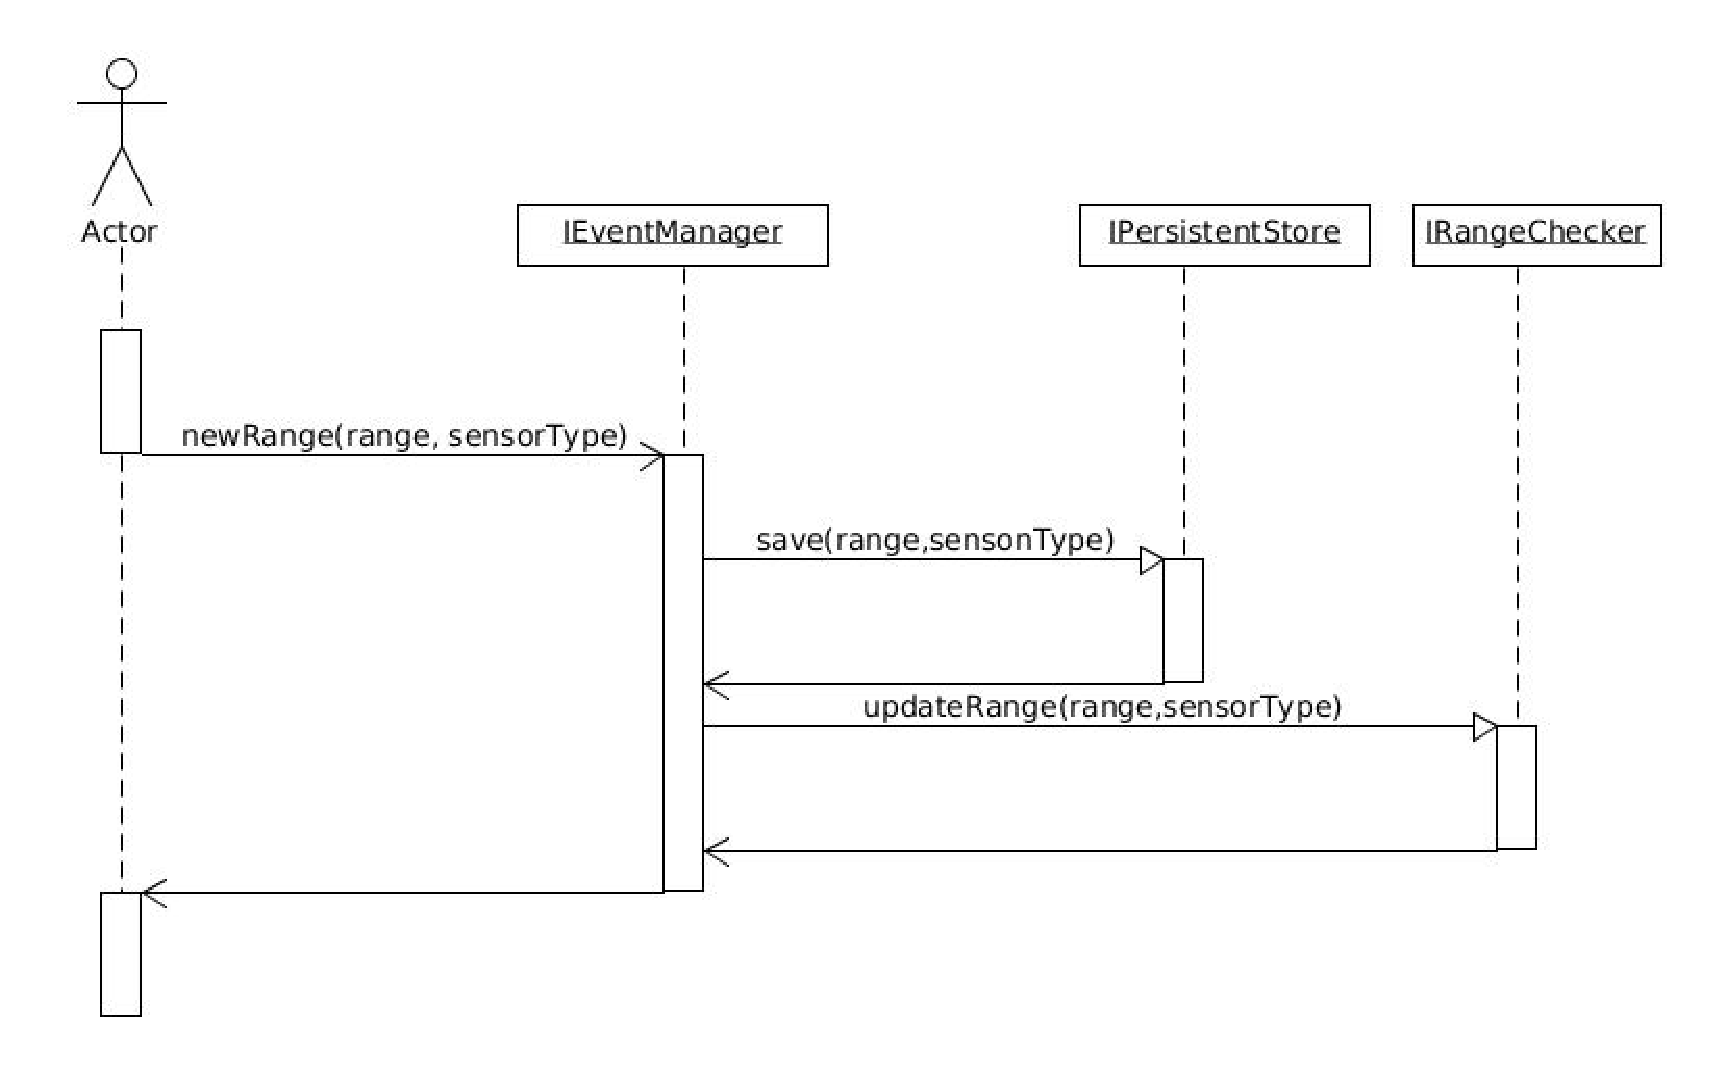
\includegraphics[scale=0.4]{Figures/DomainModel/Server/NewRangeInteraction}
\caption{Server, Interazione, Nuovo Range}
\end{figure}

In questo caso invece viene illustata l'interazione per quanto riguarda la richiesta da parte dell'utente dell'inserimento di un nuovo range. Si nota come la chiamata, questa volta, arrivi all'entit\'a che gestisce gli eventi essendo questo effettivamente un caso incui avviene un cambiamento nei dati e quindi tutto va gestito appropriatamente per evitare i conflitti.

\begin{center}
\textbf{Comportamento}
\end{center}

\begin{figure}[h]
\centering
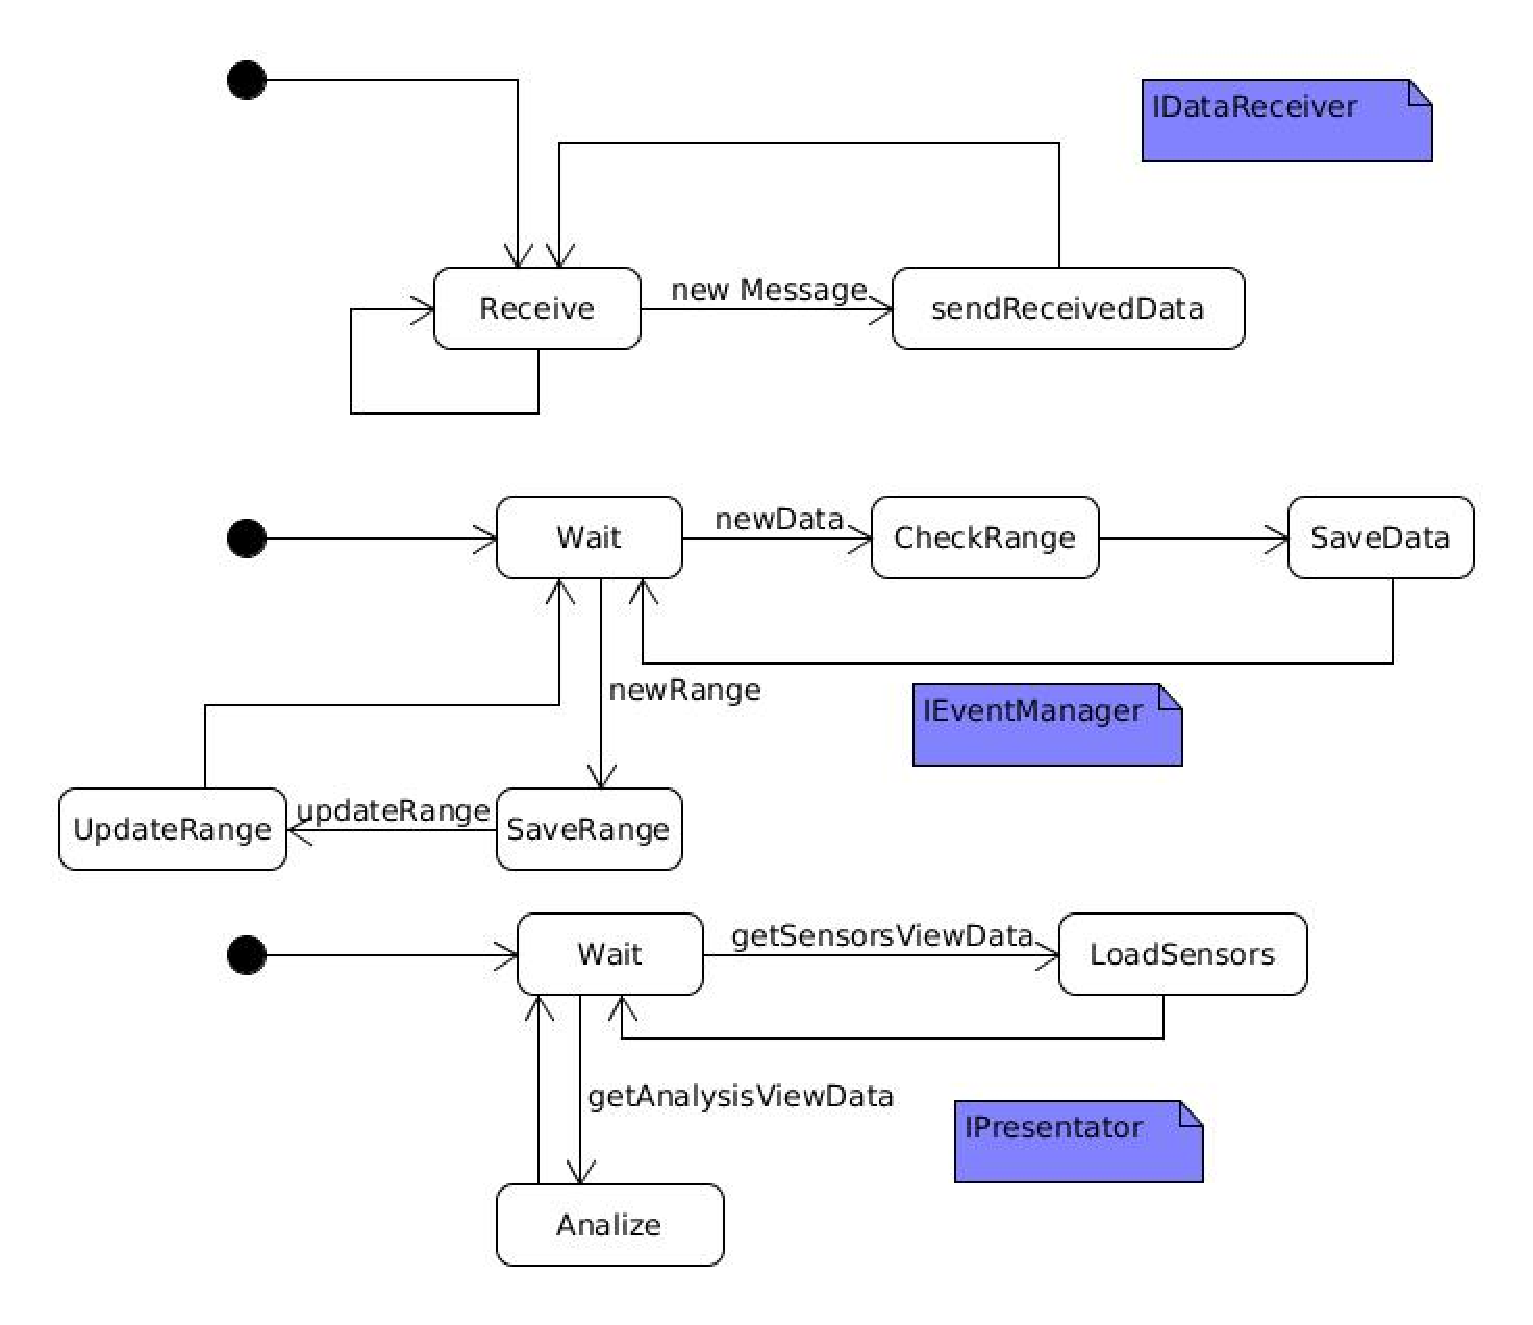
\includegraphics[width=\textwidth]{Figures/DomainModel/Server/Behaviour}
\caption{Server, Comportamento}
\end{figure}


In questa fase si mostrano le entit\'a che sono effettivamente attive e che quindi operano cambiamenti sul sistema. Si \'e deciso di omettere tutte le entit\'a che vengono solamente chiamate ed effettuano una unica operazione al fine di evitare di formalizzare troppe cose a questo livello.

Si vuole far notare inoltre come tutte queste entit\'a abbiano effettivamente uno stato di attesa di un qualche messaggio o evento. Questo aspetto pu\'o essere molto importante in seguito nelle scelte per la progettazione.

\newpage

\subsubsection{Web Site}

\paragraph{}Dopo un'attenta analisi abbiamo ritenuto superflua la necessit\'a di modellare e analizzare la parte di visualizzazione in quanto non \'e effettivamente presente nessuna business logic ma solamente la parte che effettua le richieste di dati alle parti precedenti visuzalizzando tutto su schermo.

La documentazione relativa a questa parte si limiter\'a solamente a come utilizzare il software attraverso l'interfaccia.

Possiamo pensare di definire i link a cui l'interfaccia dovr\'a rispondere appropriatamente attraverso una pagina web. Questo ci consente di impostare comunque dei test che esulano dal contenuto della pagina, garantendoci per\'o che questa sia effettivamente online in maniera automatica.

gli URL scelti sono:
\begin{itemize}
  \item \textit{http://...../DomoticRoom/Status}
  \item \textit{http://...../DomoticRoom/NewRange}
  \item \textit{http://...../DomoticRoom/Analysis}
\end{itemize}


\section{Analisi del Problema}
\labelsec{ProblemAnalysis}
%===========================================================================

\paragraph{Assunzioni}
Prima di iniziare l'analisi del problema abbiamo ritenuto neccessario effettuare delle assuzioni riguardanti al paradigma che ci consentirebbero di effettuare un prodotto di qualit\'a migliore e con meno sforzi.

Il paradigma di programmazione di riferimento \'e il \textit{reactive programming} perch\'e la concezione di flusso di dati \'e proprio quello che ci interessa modellare in quanto anche nel nostro sistema sar\'a presente un flusso di dati dal client al server. Per la comunicazione attraverso la rete questo ci consente di sfruttare chiamate asincrore aumentando il disaccoppiamento tra client e server.

Per questo abbiamo deciso di utilizzare per i dati un database NoSQL per via dell'estrema dinamicit\'a, in quanto ci consente di aggiungere dei campi anche in seguito e un miglioramento di performance nell'accesso a dati che normalmente richiederebbero dei join.

Per ulteriori informazioni pi\'u dettagliate sul paradigma si rimanda ad un'altra sede. 

\subsection{Architettura Logica}

Per la costruzione dell'architettura logica ci si baser\'a ovviamente sulla precedente analisi dei requisiti in modo da mantenere il contatto con questi e non rischiare di uscire fuori specifica. Anche in questo caso si andr\'a separare l'analisi in due parti:

\begin{itemize}
\item Sistema Embedded
\item Server e Website
\end{itemize}

La parte del website \'e stata incorporata direttamente nella parte server proprio per la sua assenza di business logic.

\paragraph{Modellazione Reactive}

Prima di iniziare a costruire la modellazione sulla base del paradigma appena citato \'e necessario capire come fare a modellare lo stream stesso all'interno della nostra architettura logica, conseguentemente si \'e deciso di utilizzare i \textit{marable diagrams}. Questi sono una rappresentazione di come il flusso di dati nel tempo avviene e quali tipologie di trasformazioni consentono di effettuare.

Con questi schemi ci viene concesso ancora una volta di concentrarci prima sul ''cosa'' e non sul ''come'' che invece viene delegata alla parte progettuale, dove si cercher\'a effettivamnete di implementare il risultato finale dell'analisi

\subsubsection{Sistema Embedded}

\begin{center}
  \textbf{Flussi Dati}
\end{center}

Alla luce del paradigma di programmazione che si \'e deciso di adottare sono stati effettuati dei cambiamenti anche alla struttura che \'e stata esposta precedentemente proprio perch\'e ci sono state fornite da questa assunzione nuovi livelli di astrazione, primo tra tutti il concetto di \textbf{Stream/Flusso}. Quindi in questa fase abbiamo ritenuto molto utile iniziare a visualizzare effettivamente questi flussi tramite un'apposito diagramma.

% Figura fatta con draw.io
\begin{figure}[ht]
\centering
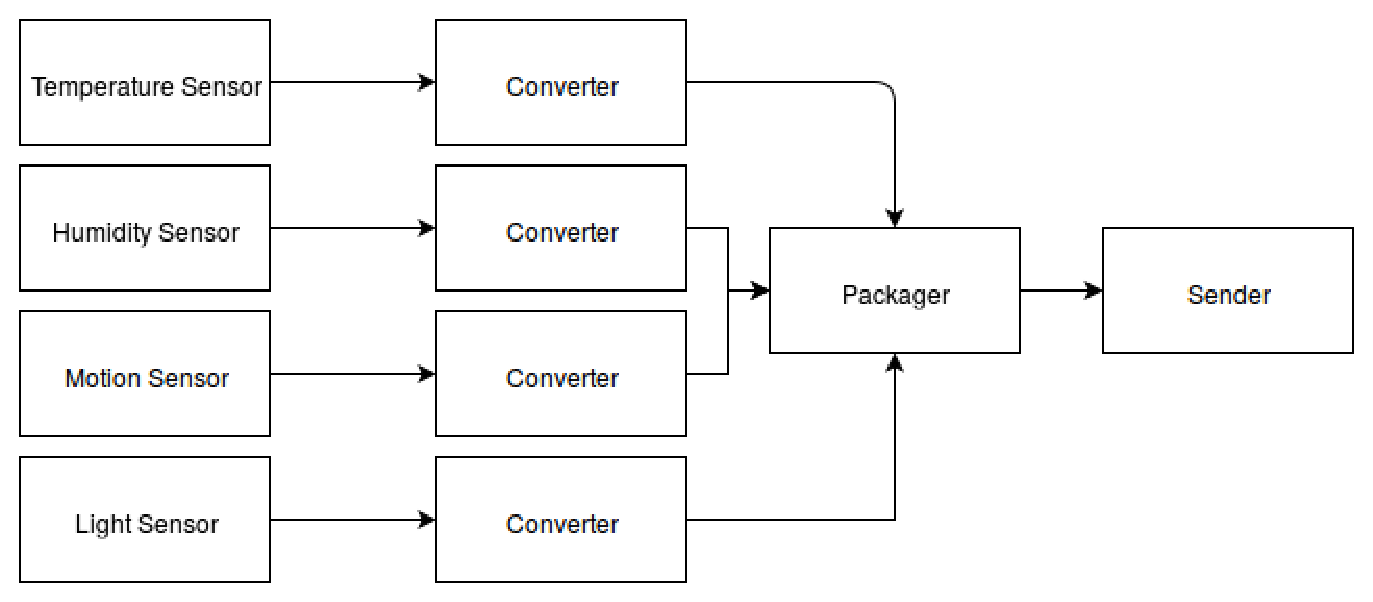
\includegraphics[width=\textwidth]{Figures/LogicArchitecture/EmbeddedSystem/FlowDiagram}
\caption{Diagramma di flusso, per sensore, dei dati}
\end{figure}


In particolare si puo' notare come in questo diagramma il compito di convertire i valori di un sensore sia stato disaccoppiato dal sensore stesso che quindi si deve solamente occupare di invitare i dati all'interno del flusso. \'E stato inoltre aggiunto anche una nuova entit\'a \textit{packager} che si occuper\'a di formattare i valori secondo il protocollo che deve essere definito tra client e server per l'apposita comunicazione. In particolare ogni dato proveniente da un sensore avr\'a un suo formato per via: della differenziazione dei dati, della tempistica di rilevazione che pu\'o anche risultare diversa e dell'idea percui la comunicazione in ogni caso debba essere asincrona.

Sulla base di questa ultima frase si vuole sottolineare che ogni sensore quindi avr\'a un suo flusso asincrono, ma che in quest'immagine si \'e deciso di condensare in un'unica immagine per comodit\'a.

Di seguito si indica un primo marable diagram che mostra le varie trasformazioni che verranno applicate. Questo serve soprattutto per iniziare a capire poi come interpretare eventuali altri schemi come questo.

% Figura fatta con draw.io
\begin{figure}[ht]
\centering
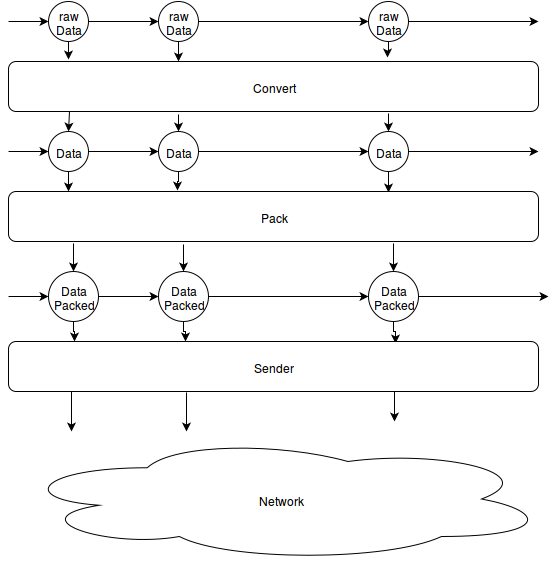
\includegraphics[scale=0.7]{Figures/LogicArchitecture/EmbeddedSystem/MarableDiagram}
\caption{Marable diagram dei singoli dati proveniente da una sorgente}
\end{figure}


\afterpage{\clearpage}

\newpage

\begin{center}
  \textbf{Struttura}
\end{center}

Chiaramente la struttura, che si basa sul precedente step di analisi dei requisiti, risulta cambiata anche alla luce delle assunzioni effettuate e quindi si possono notare l'introduzione di alcune entit\'a che servono per la gestione del sistema embedded e per impostare i flussi di dati provenienti dai sensori.

\begin{figure}[h]
\centering
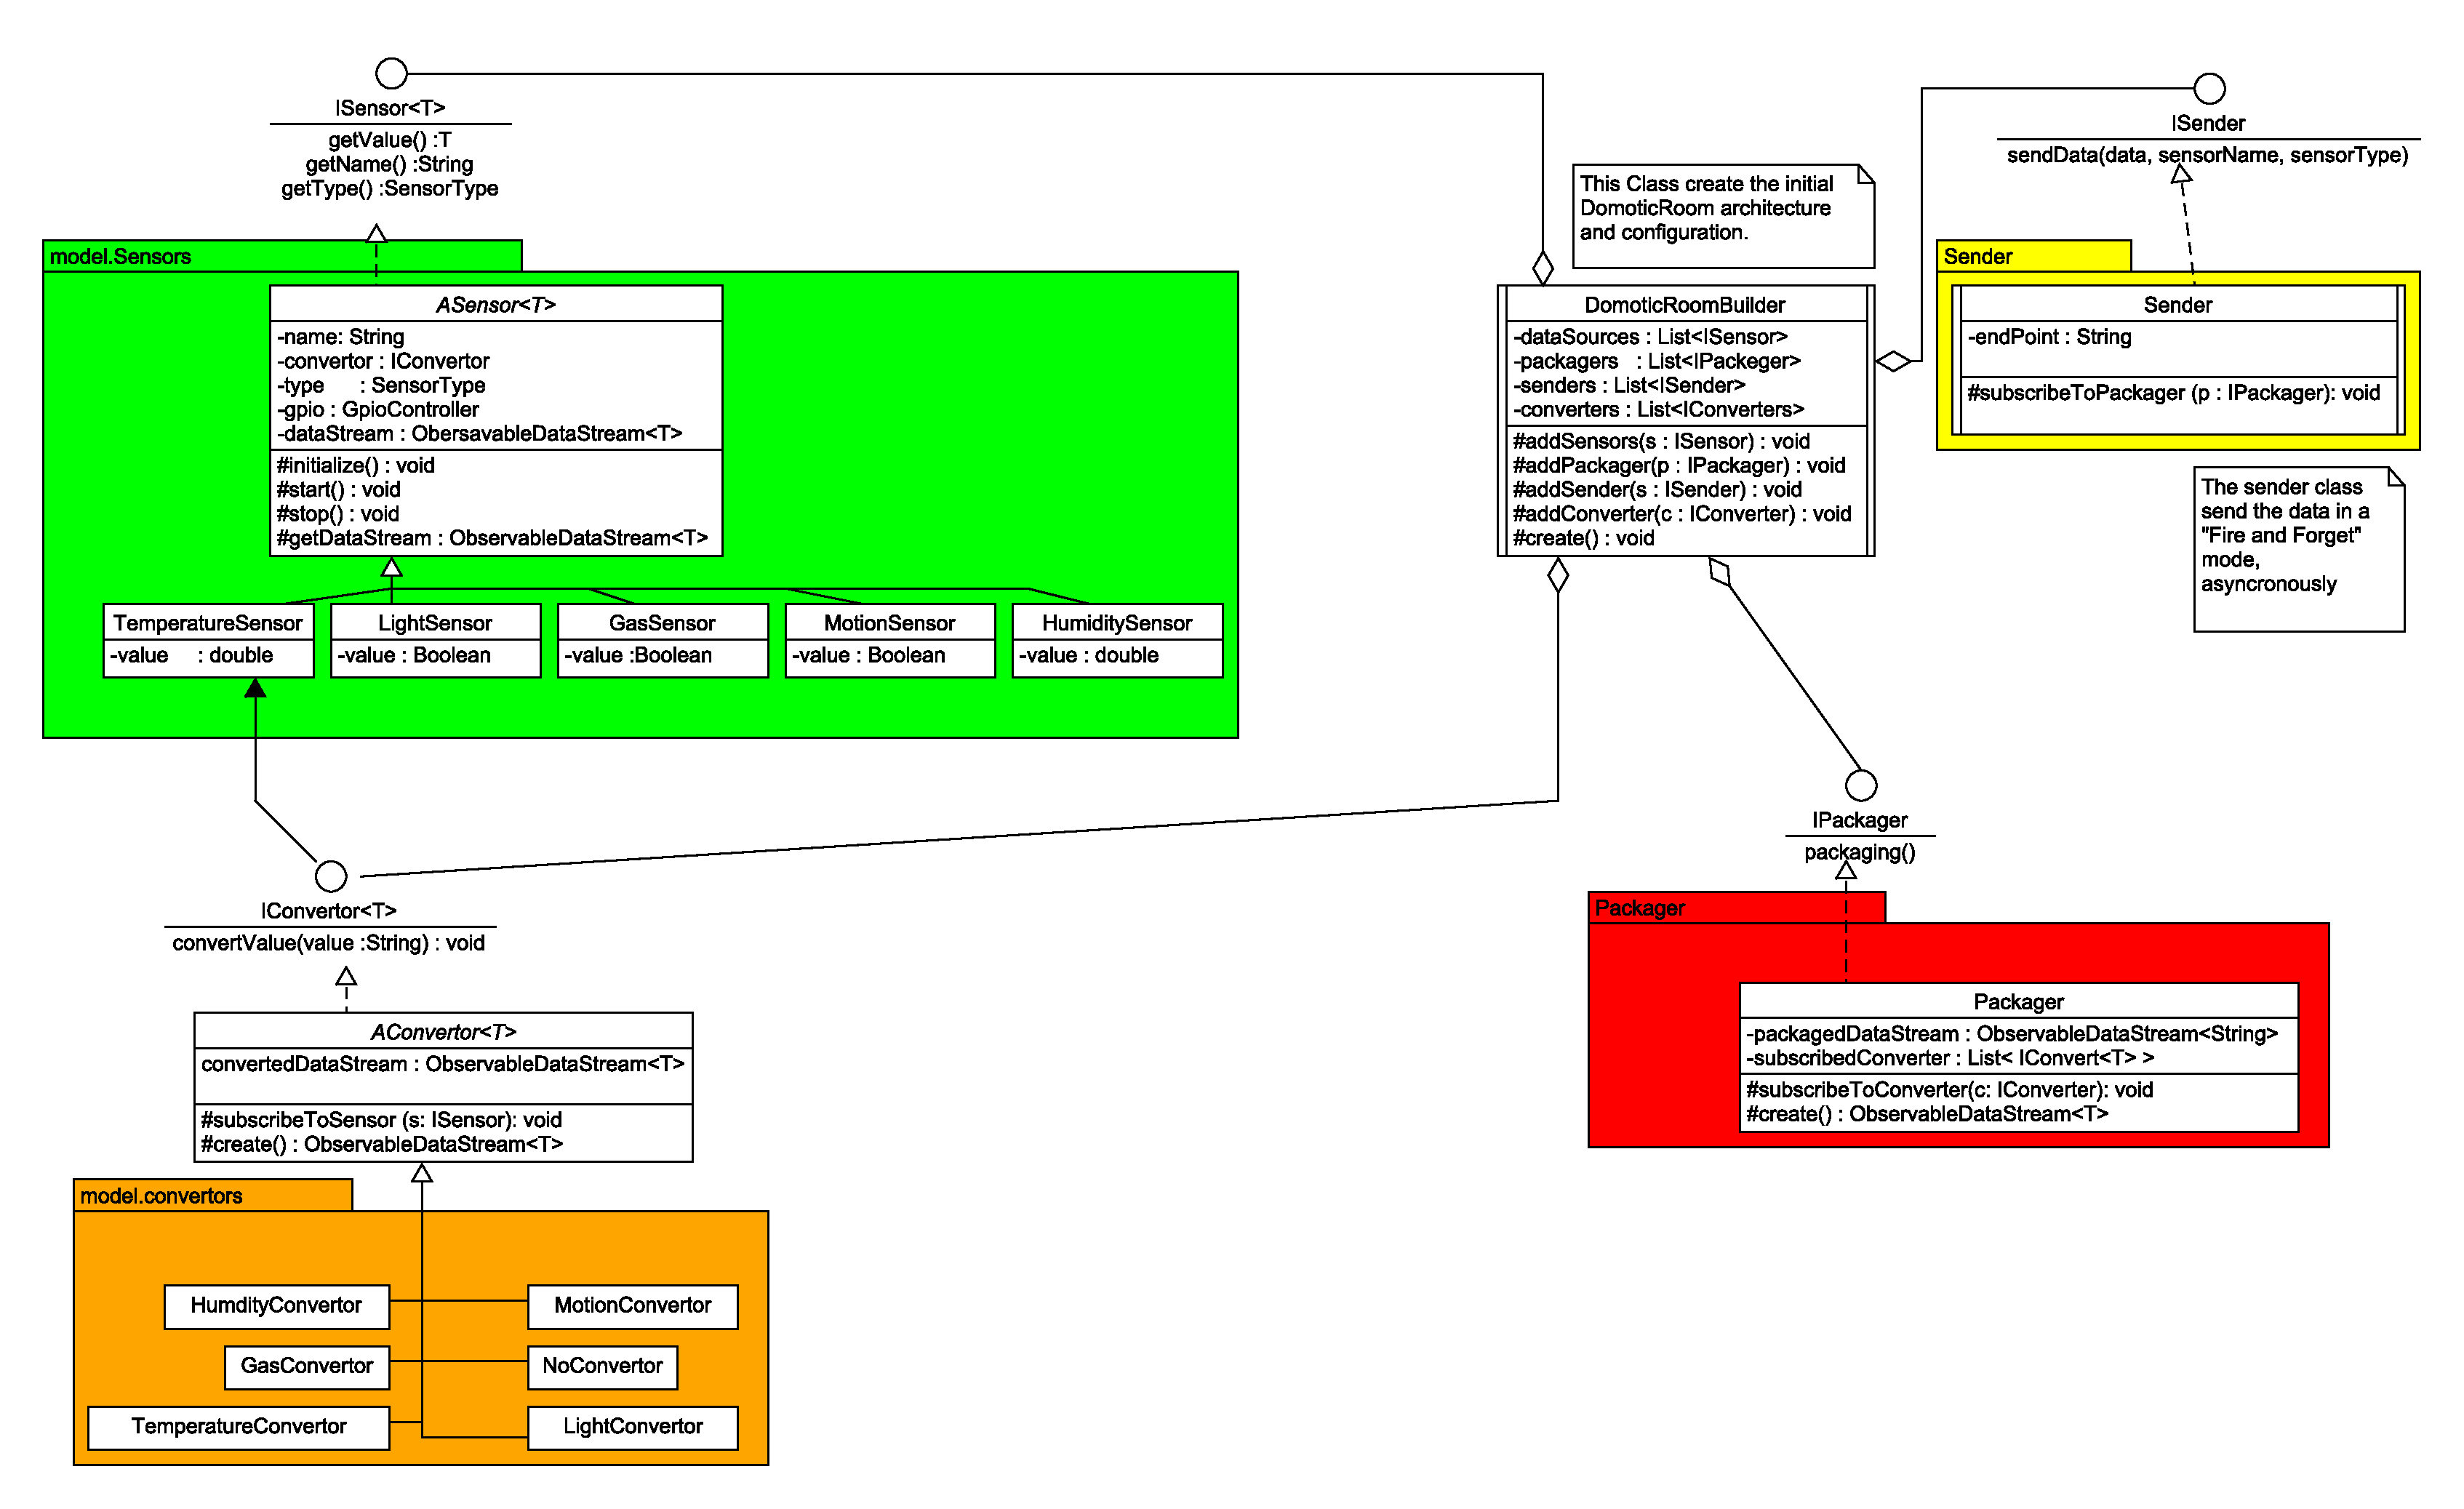
\includegraphics[scale=0.2]{Figures/LogicArchitecture/EmbeddedSystem/Structure}
\caption{Logic Architecture, Structure}
\end{figure}

Come si mostra nello schema soprastante, la struttura logica non ne esce particolarmente modificata rispetto all'analisi iniziale.\\
Il \textit{SensorDataFetcher} è stato eliminato, poich\`e l'implementazione di polling per ricevere dati dai sensori viene sostituita dal pattern Observable, utilizzato per sfruttare tutte le potenzialità del paradigma Reactive. \\
La nuova entit\'a \textit{DomoticRoomBuilder} ha il ruolo centrale di inizializzare il sistema, creando l'architettura e la configurazione iniziale dei suoi componenti.\\
L'entit\'a \textit{Sensor} ha il ruolo centrale di ricevere i dati dai sensori e inviarli su uno stream dati osservabile.
L'entit\'a \textit{Convertor} si occupa di convertire i dati che riceve dalla sorgente \textbf{Sensor} a cui è sottoscritto; inoltre genera un nuovo Stream dove invia i dati convertiti che riceve dai \textit{Sensor} a cui è sottoscritto.\\
L'entit\'a \textit{Packager} unisce tutti i flussi in entrata, dai \textit{Converter} in un unico flusso, il suo compito è preparare i dati ad essere inviati al Server.\\
L'entit\'a \textit{Sender} si occupa di inviare i dati che riceve dal Packager sulla rete, come pensato nella struttura iniziale.

\begin{center}
  \textbf{Interazione}
\end{center}

La parte di interazione viene drasticamente modificata proprio perch\'e l'assunzione del paradigma reactive risulta principalmente improntato su questo, in particolare \'e possibile condensare in meno codice, e pi\'u dichiarativo. Vengono in ogni caso mostrati le varie operazioni effettuate sullo stream per mantenere il contatto con quanto mostrato attraverso i marable diagrams. Particolare attenzione va posta poi sulla parte che converte da \textit{procedure calls} a \textit{reactive streams}. \\
Il sistema non ha una interazione continua; come invece suggerisce il paradigma, esso "reagisce" al verificarsi di un evento di particolare interesse.\\
In questo caso, il sistema reagisce autonomamente alla ricezione di un valore inviato dal sensore. L'entit\'a \textit{Sensor} si occupa di incanalare queste letture periodiche in un flusso potenzialmente infinito di valori.\\
L'entit\'a \textit{Convertor} \'e a sua volta interessata all'arrivo di un nuovo valore sul flusso creato dal \textit{Sensor}; il Convertor applicher\'a ad ogni nuovo dato una funzione atta a convertire in valore in un dato di maggiore utilità per il sistema.\\
L'entit\'a \textit{Packager} sarà invece di ascolto sui flussi generati da ogni \textit{Convertor}, appena un nuovo valore convertito è inviato sul flusso; a questo punto il suo compito \'e "impacchettare" il dato, secondo un protocollo di trasmissione per poterlo inviare al Server.\\
Quest'ultima parte \'e gestita dal \textit{Sender} che appena un dato impacchettato \'e pronto lo invier\'a al Server.

\begin{center}
\textbf{Comportamento}
\end{center}

\subsubsection{Server}

\begin{center}
  \textbf{Interazione e Flussi Dati}
\end{center}

Anche per quanto riguarda la parte server \'e necessario definire gli steam che saranno presenti all'interno del sistema. Inquanto questa parte \'e notevolmente pi\'u corposa rispetto a quella dell'embedded system per varie ragioni, prima tra tutte la capacit\'a di calcolo, saranno necessari pi\'u stream, in particolare si \'e pensato di creare uno stream per ogni funzionalit\'a sulla base delle operazioni che quindi sono da compiere.

Il primo flusso che andremo ad analizzare riguarda la ricezione dei dati da parte del sistema embedded. In particolare si vuole cercare di riutilizzare le entit\'a che si sono introdotte nell'analisi dei requisiti proprio perch\'e queste sono maggiormente collegate al dominio. Si pu\'o inoltre notare altre entit\'a chiamate \textit{IRawDataFormatter e IDBDataFormatter}, queste entit\'a sono utili per preparare la corretta formattazione dei dati e la loro validazione, provenienti dal flusso e dalla successiva elaborazione per essere salvati poi sul database. Si \'e deciso in particolare di inserirlo per andare a separare i compiti il pi\'u possibile e per facilitare la modifica nel caso si voglia adottare uno standard dei dati interno rispetto a quello del client in modo da effettuare una netta indipendenza tra server e client. Soprattutto perch\'e in un'eventuale futuro si pu\'o facilmente immaginare un'eterogeneit\'a dei dati dovuti ai vari client disponibili e dalla loro provenienza (altre aziende, protocolli proprietari \ldots)

\begin{figure}[h]
\centering
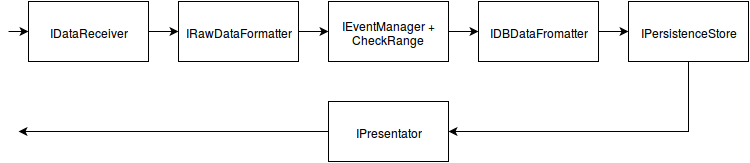
\includegraphics[width=\textwidth]{Figures/LogicArchitecture/Server/FlowDiagramReceiveData}
\caption{Server, Flusso Dati Ricezione}
\end{figure}

Il secondo e ultimo flusso di dati che verr\'a trattato riguardano le richieste di dati stessi per la visualizzazione da parte dell'utente. Probabilmente per quanto riguarda le seguenti operazioni si poteva anche pensare di gestire il tutto attraverso delle semplici chiamate a procedura, ma, per mantenere una certa coerenza, per sfruttare la dichiarativit\'a del paradigma reactive e per evitare di incorrere nel problema noto come \textit{Callback Hell} si \'e scelto di utilizzare comunque un flusso. Un'ulteriore vantaggio di gestire attraverso l'infrastruttura reactive consiste nella possibilit\'a di aggiornare realtime l'interfaccia ogni qualvolta avviene l'inserimento di un nuovo valore. Concludendo si vuole far notare la presenza di un'entit\'a che entra in campo quando viene richiesta un'analisi sui dati e non semplicemente una sua visualizzazione. La forma a nuvola indica proprio la possibilit\'a che questo oggetto entri a far parte o meno nel flusso.

\begin{figure}[h]
\centering
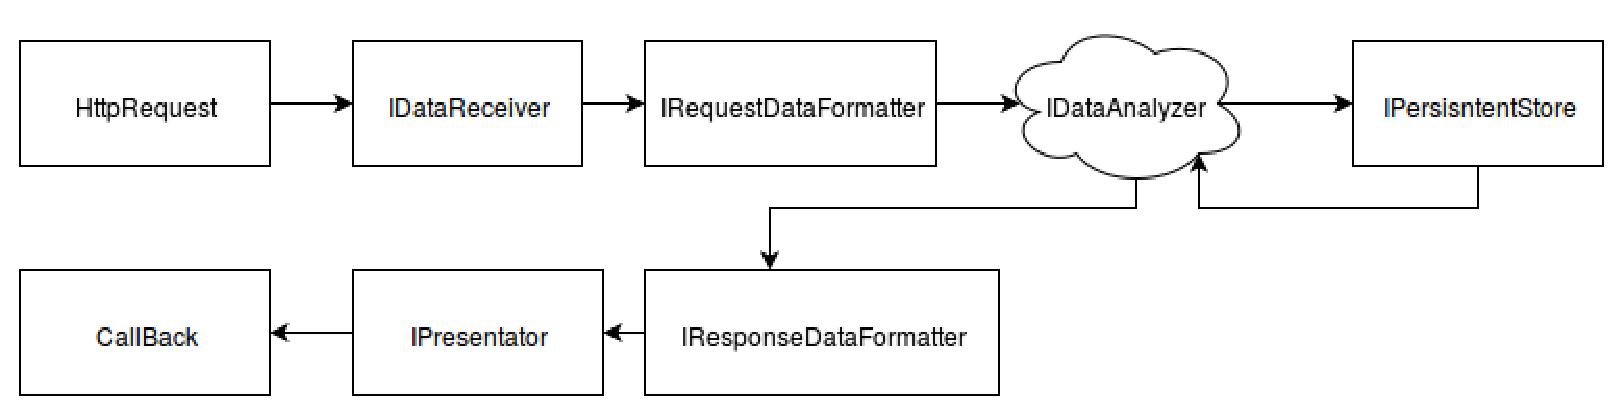
\includegraphics[width=\textwidth]{Figures/LogicArchitecture/Server/FlowDiagramViewData}
\caption{Server, Flusso Dati Richieste Dati}
\end{figure}

\begin{center}
  \textbf{Restanti Interazioni}
\end{center}

Per quanto riguarda  riguarda l'aggiornamento del range da parte dell'utente, in particolare anche in questo caso l'IEventManager viene chiamato in causa il quale si occuper\'a di notificare il cambiamento sia a livello di database che al componente incaricato di controllare il range. Questa parte non subisce particolari cambiamenti rispetto a quella dell'analisi dei requisiti perch\'e rimane molto coerente anche a fronte del cambio di paradigma. Un cambiamento significativo riguarda il fatto che il cambiamento del range non avviene pi\'u direttamente dall'event manager ma dal database, questo per enfatizzare che il cambiamento del range non \'e effettivo se non viene prima registrato in maniera permanente.

Questa interazione non avviene attraverso uno stream ma viene gestito come una chiamata classica http in quanto non richiede che ci sia un dialogo continuo tra le varie parti, client e server. Si riporta in ogni caso sotto forma di flusso di chiamate, quelle che vengono effettuate dall'applicativo.

\begin{figure}[h]
\centering
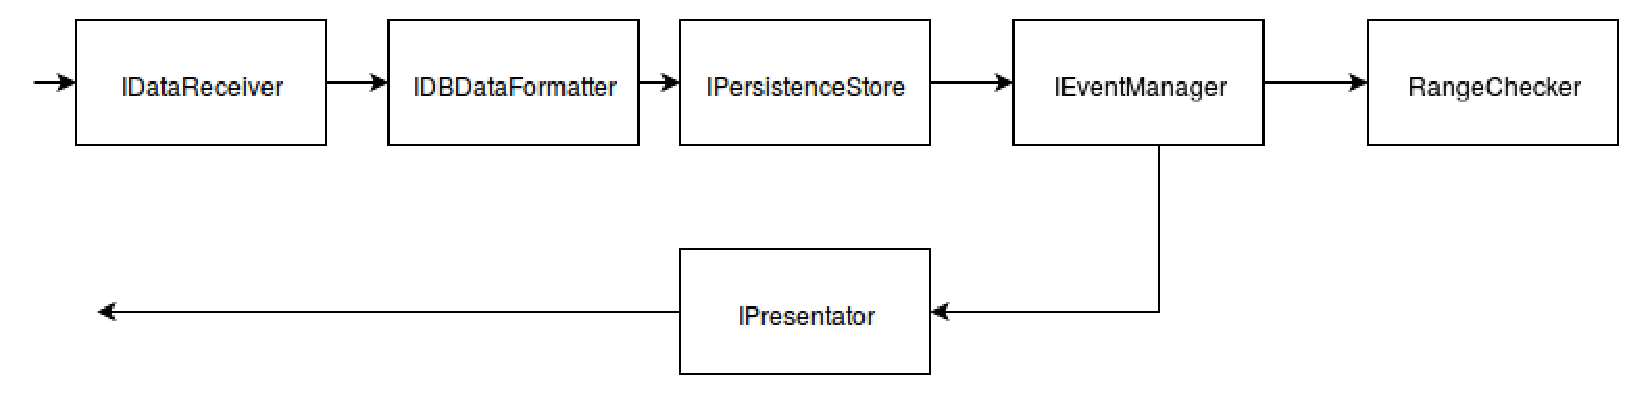
\includegraphics[width=\textwidth]{Figures/LogicArchitecture/Server/FlowDiagramNewRange}
\caption{Server, Flusso Dati Nuovo Range}
\end{figure}

\newpage

Prima di passare alla struttura \'e secondo noi utile andare a definire l'interazione del configurator in quanto \'e l'unica entit\'a attiva che non si basa effettivamente sui flussi e che contiene l'entry point di tutto il server.

\begin{figure}[h]
\centering
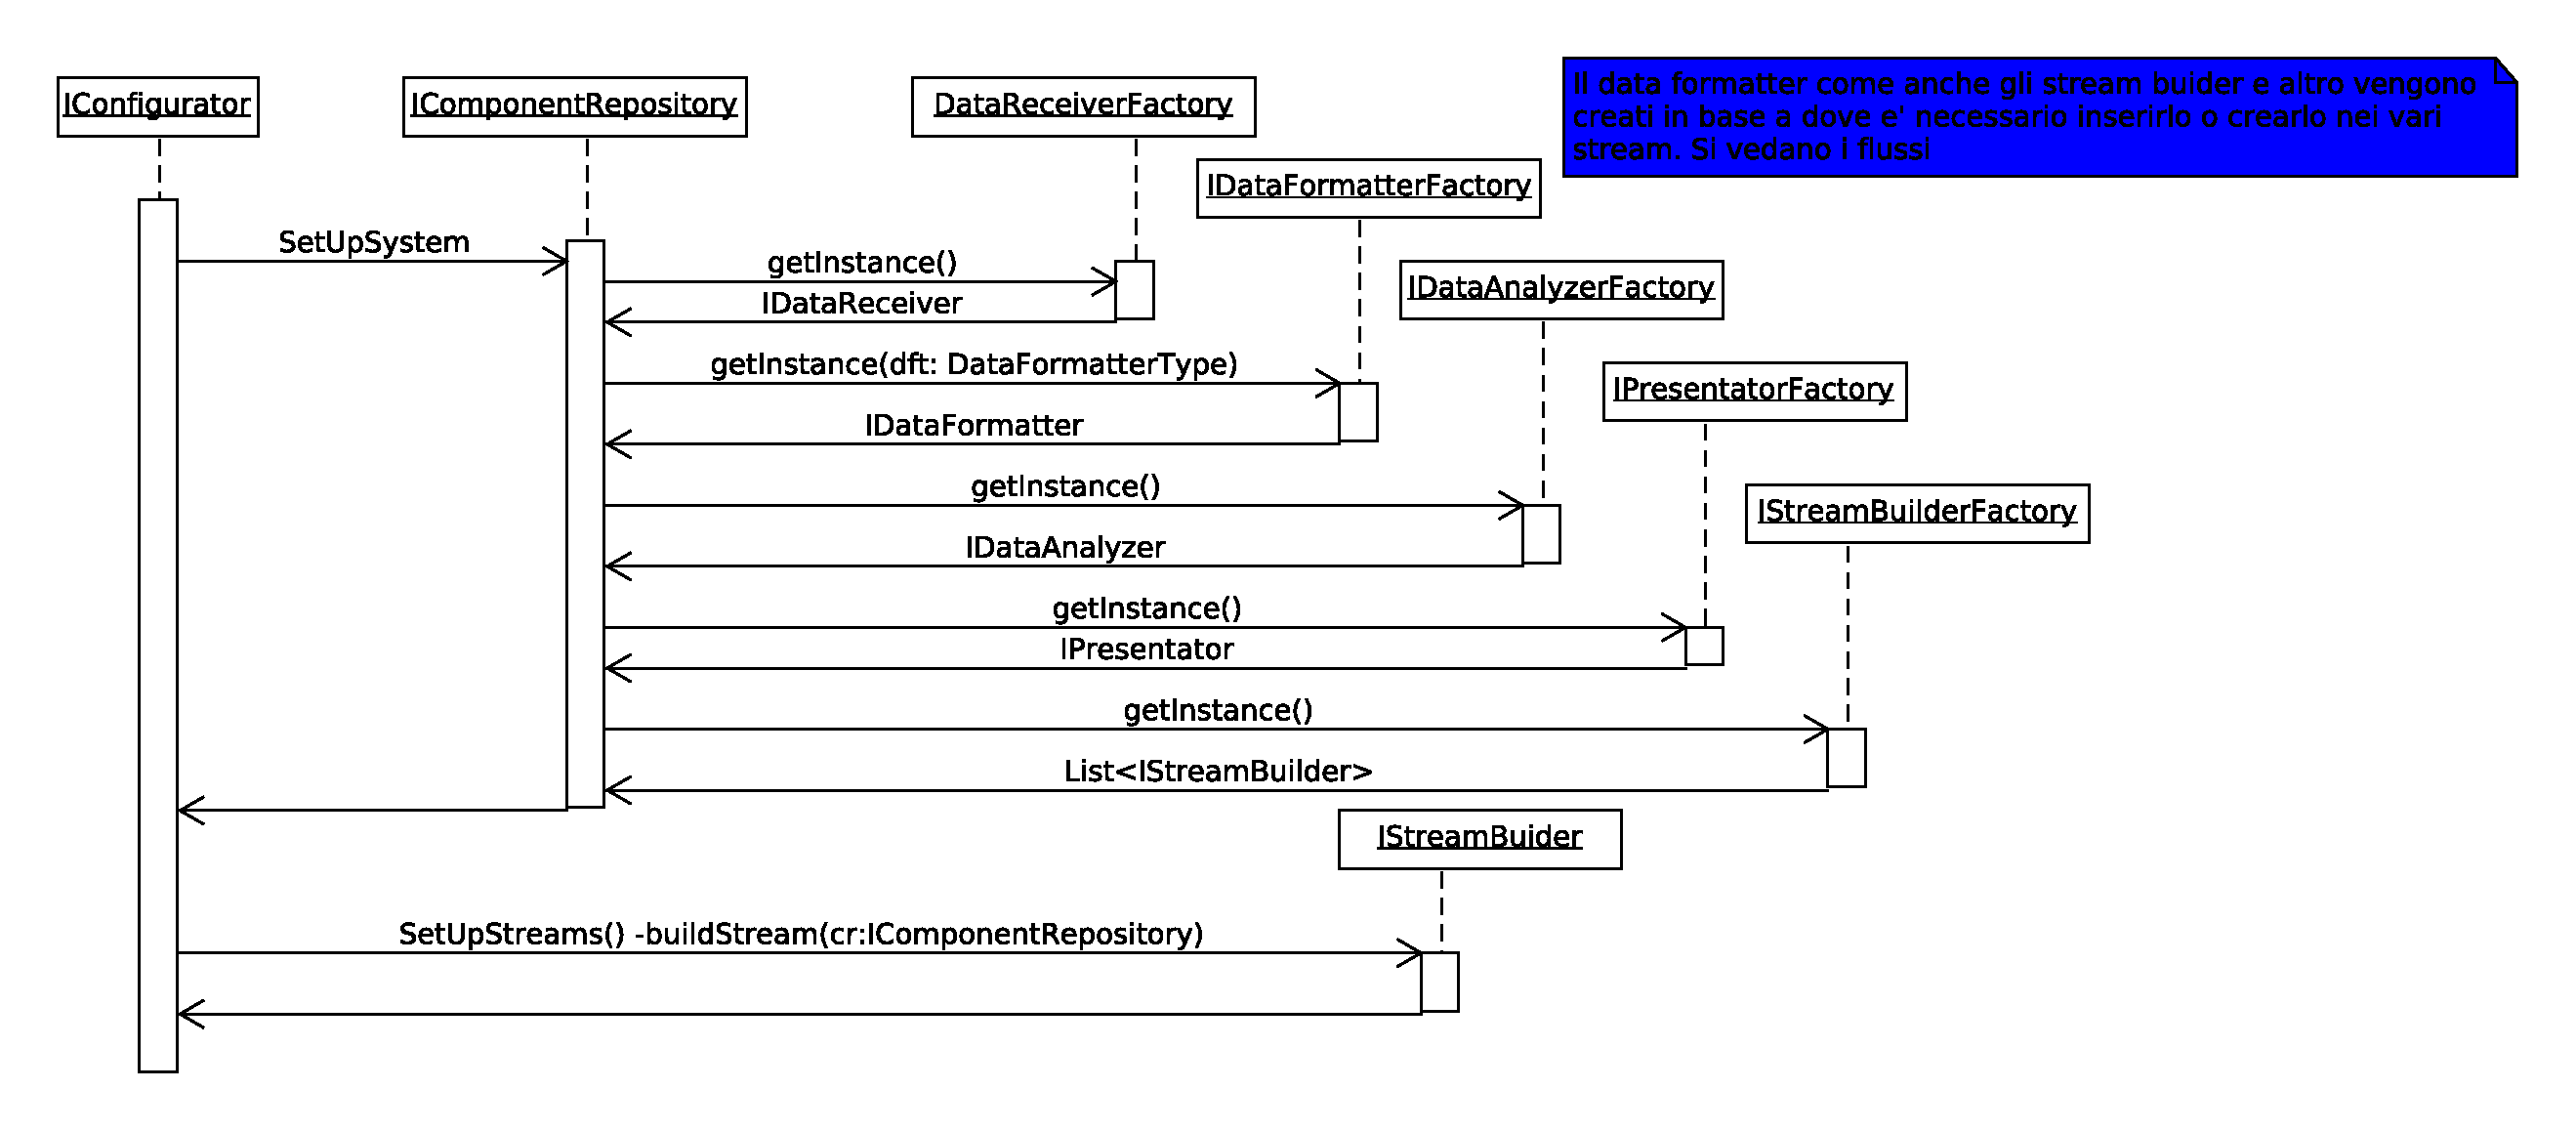
\includegraphics[width=\textwidth]{Figures/LogicArchitecture/Server/IConfiguratorInteraction}
\caption{Server, IConfigurator Interaction}
\end{figure}

\newpage

\begin{center}
\textbf{Struttura}
\end{center}

Nella struttura dell'analisi del problema abbiamo varie differenze, anche a livello di interfaccia, dovute al cambio di paradigma o ad altre motivazioni, di seguito verranno elencate per rendendere tutto pi\'u chiaro:

\begin{itemize}
\item IDataReceiver: non esiste pi\'u il metodo \textit{Receive} perch\'e non si ipotizza pi\'u un'approccio a polling e quindi non \'e necessaria questa funzionalit\'a, mentre invece viene esposto un metodo che da la possibilit\'a di ottenere lo stream di dati associato all'arrivo di un nuovo valore dall'esterno.
\item Tutto ci\'o che in precedenza, nel diagramma dell'interazione, era modellato attraverso una chiamata a procedura e veniva effettuata all'arrivo di un nuovo dato, ora viene convertito in funzioni che prendono in ingresso un dato stream e lo modificano restituendo un nuovo stream all'inizio del sistema in modo che, in questa fase, si \'e in grado di costruire e comporre i vari flussi che poi verranno elaborati attraverso l'infrastruttura.
\item Per separare ancora di pi\'u i vari flussi di stream indicati precedentemente e per separare i compiti di creazione dei vari stream si sono ideate delle classi \textit{factories} che assembleranno i vari componenti a tale scopo.
\item Sono stati impostati come oggetti sigleton i componenti \textit{EventManager e PersistenceStore}
\item \'E stato ampliato la parte del persistenceStore in modo da differenziare i vari compiti di salvataggio e caricamento attraverso diversi oggetti.
\item Il DataReceiver \'e stato differenziato tra dati provenienti dai sensori e dati provenienti dall'utente, come le richieste di un nuovo range o la richiesta di dati. Questo ha di fatto portato all'eliminazione dell'oggetto presentator individuato precedentemente.
\end{itemize}

\begin{sidewaysfigure}[h]
\centering
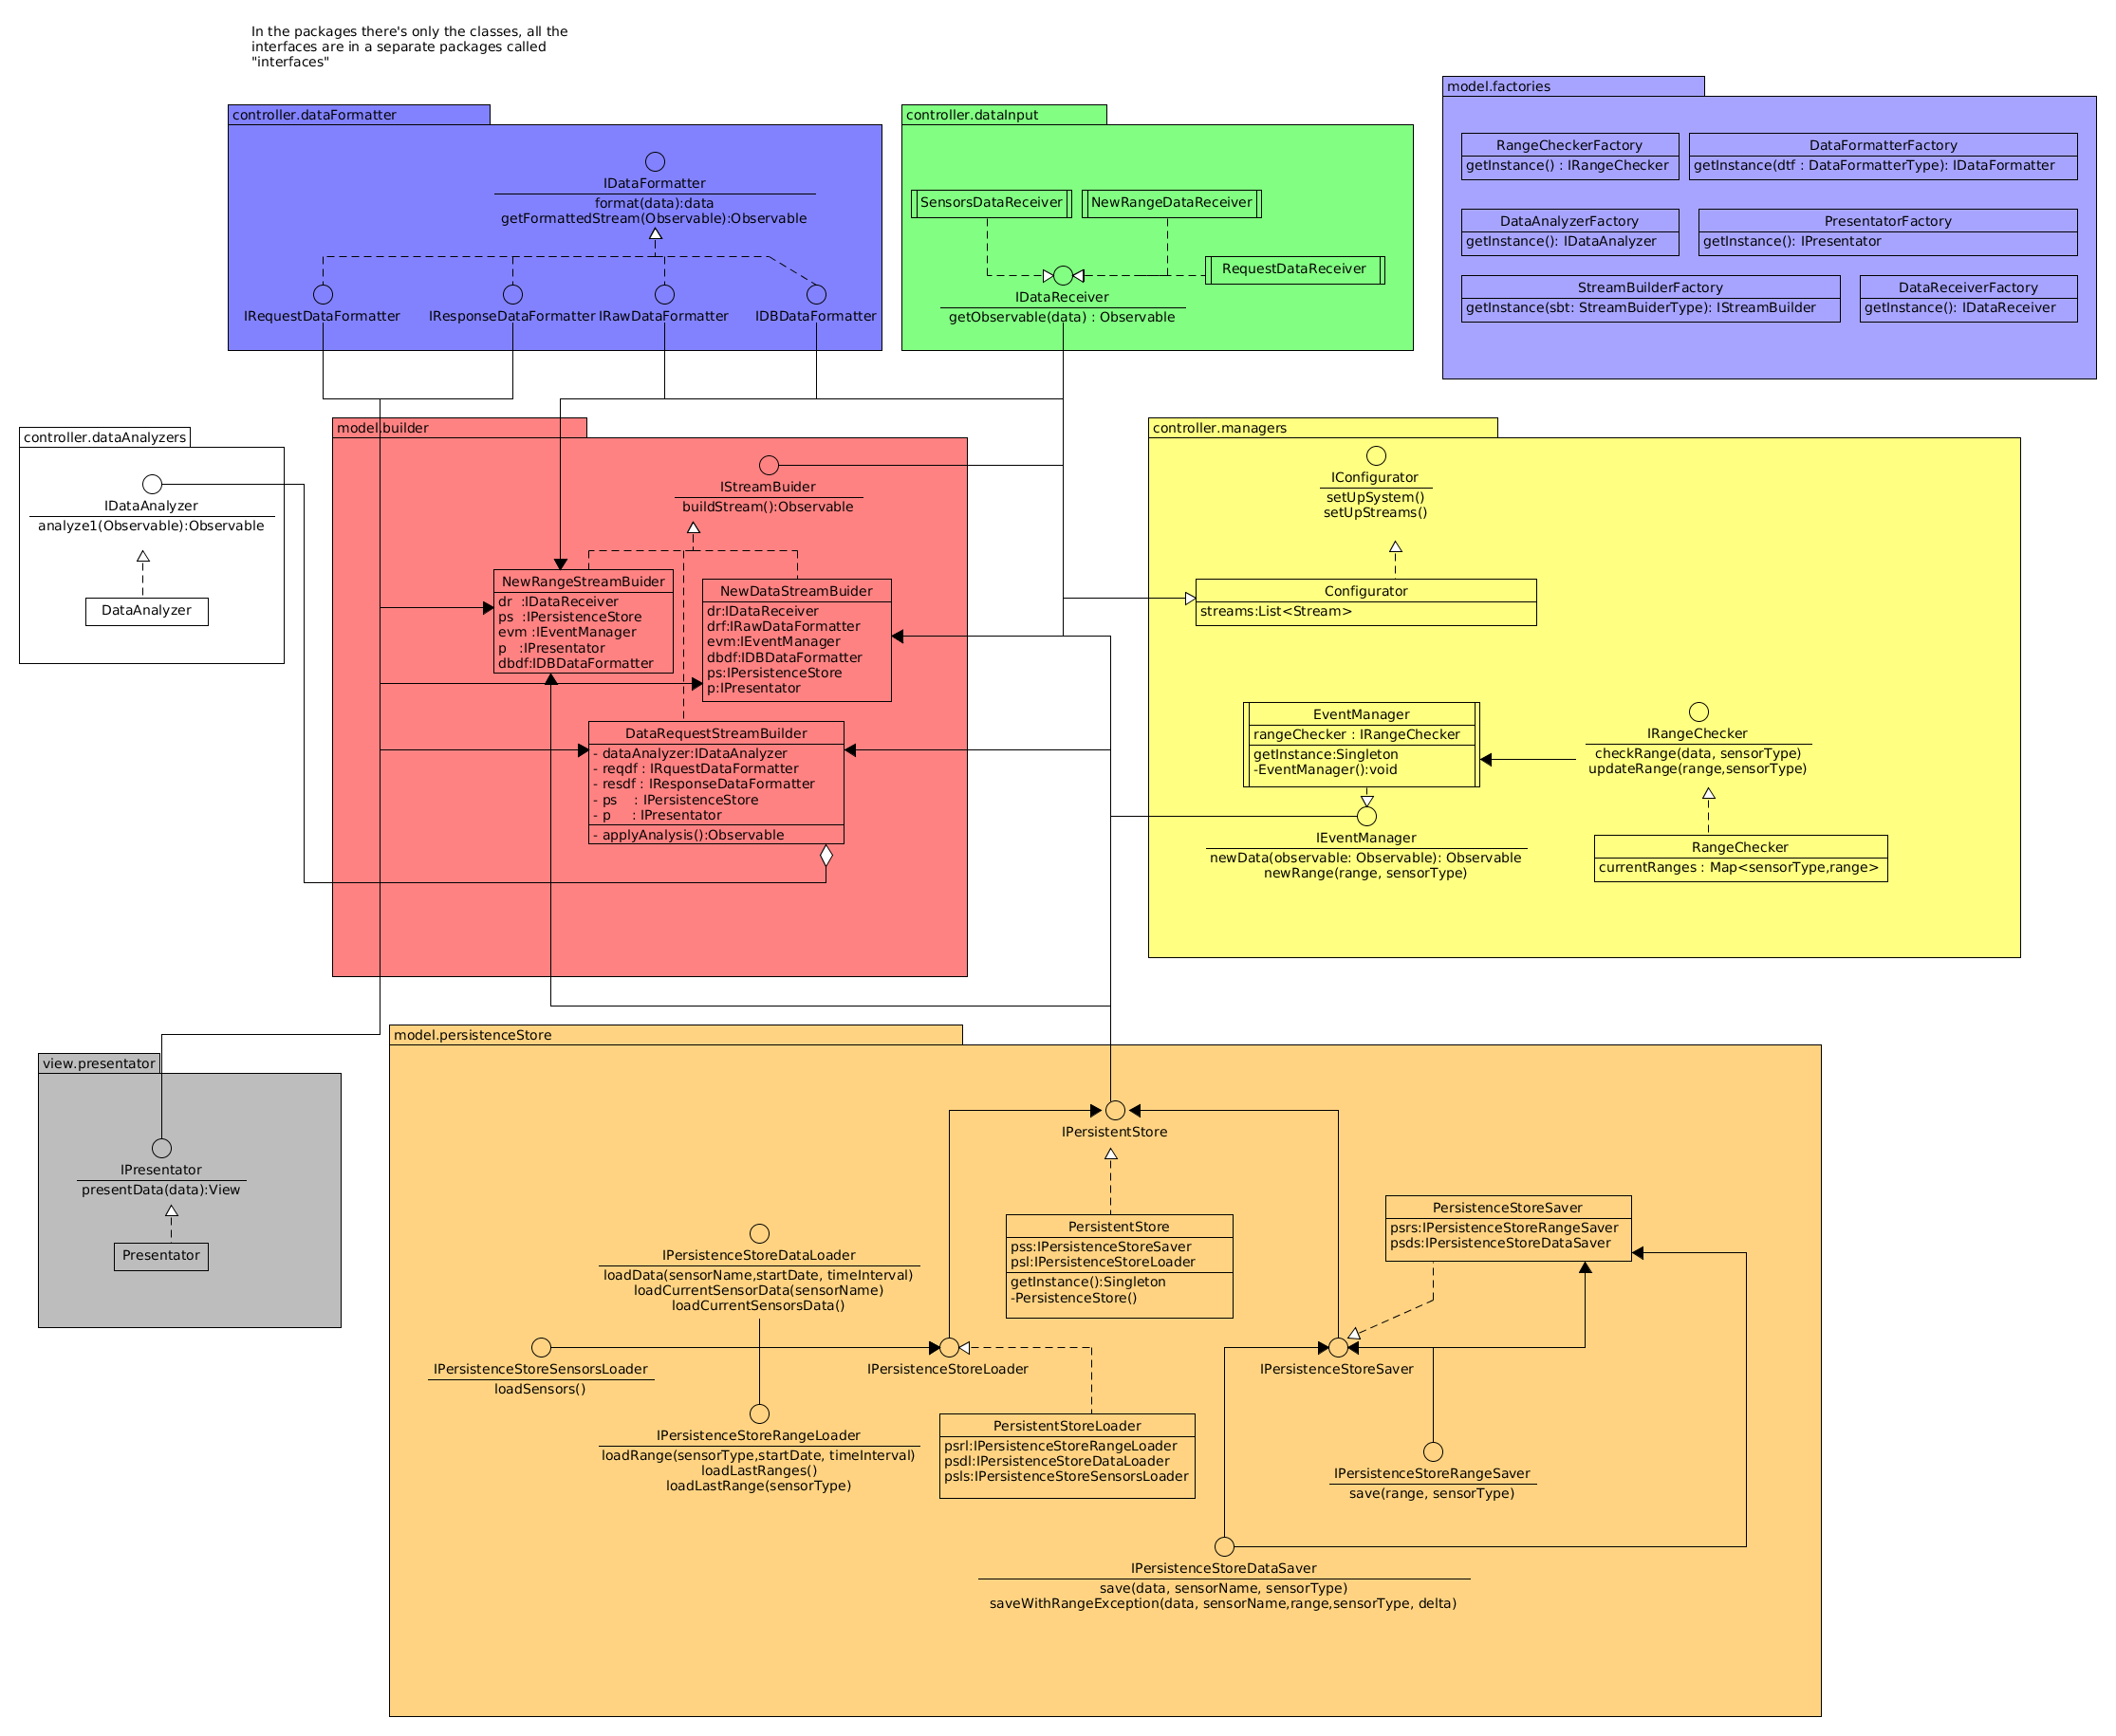
\includegraphics[width=\textwidth]{Figures/LogicArchitecture/Server/Structure}
\caption{Server, Struttura Architettura Logica}
\end{sidewaysfigure}

\afterpage{\clearpage}

\newpage

\begin{center}
\textbf{Comportamento}
\end{center}

Per quanto riguarda il comportamento delle varie parti del sistema verranno illustrate quelle principali e descritti gli stati principali incui questi componenti verranno a trovarsi. In particolare verranno omessi tutti quei componenti che effettivamente si occupano solamente della trasformazione degli stream in quanto non posseggono effettivamente uno stato, ma consistono in degli algoritmi che, dato un flusso in ingresso, gli applicano delle apposite trasformazioni e restituiscono un flusso in uscita.

\begin{figure}[h]
\centering
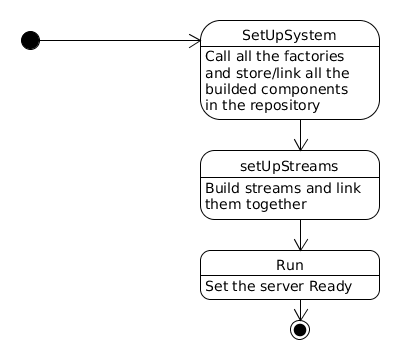
\includegraphics[scale=0.5]{Figures/LogicArchitecture/Server/IConfiguratorBehavior}
\caption{Server, IConfigurator Behavior}
\end{figure}

Come si pu\'o vedere dalla figura sovrastante il componente IConfigurator sar\'a quello che si occuper\'a di attivare tutto il sistema server occupandosi di rendere tutto operativo e pronto per le richieste da soddisfare. Questo avviene appunto in fasi, incui prima viene settato il tutto attraverso una fase di creazione di tutti i componenti necessari, poi avviene la creazione dei flussi che si occuperanno del flow dei dati ed infine si attiveranno questi flussi in modo che siano attivi.

\begin{figure}[h]
\centering
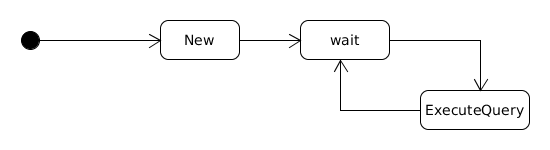
\includegraphics[width=\textwidth]{Figures/LogicArchitecture/Server/IPersistenceStoreBehavior}
\caption{Server, IPersistenceStore Behavior}
\end{figure}

Il comportamento del persistence store rimane molto semplice: una volta creato, attende la richiesta da parte del sistema per la memorizzazione dei dati.
Quando una richiesta avviene allora si attiva una delle parti che si occupano di leggere o scrivere all'interno del persistence store e effettuano l'operazione, per poi tornare in attesa di ulteriori operazioni. Si aggiunge inoltre che questo componente come l'eventManager sono componenti singleton, e quindi \'e presente solamente un'istanza di questo in tutto il sistema.

\begin{figure}[h]
\centering
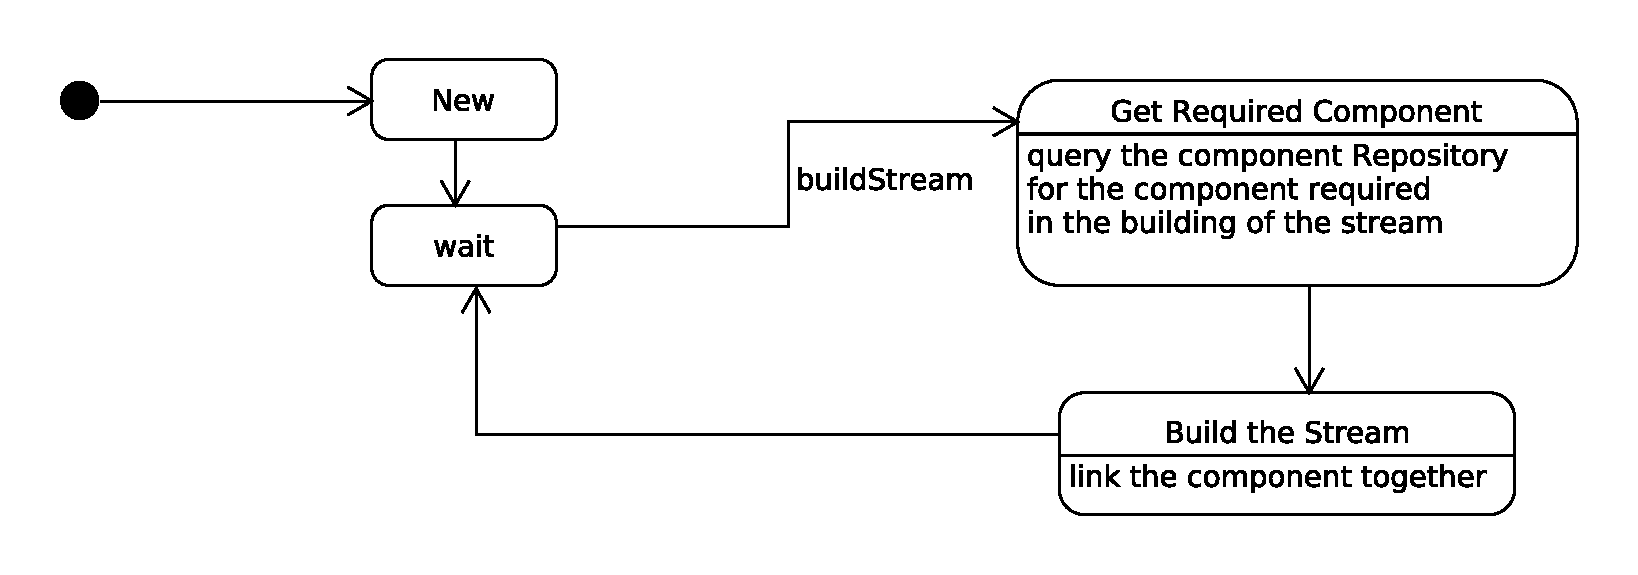
\includegraphics[width=\textwidth]{Figures/LogicArchitecture/Server/IStreamBuiderBehavior}
\caption{Server, IStreamBuilder Behavior}
\end{figure}

Lo stream builder anch'esso risulta molto semplice perch\'e viene chiamato da altri componenti, nel suo caso dal configurator stesso, e per questo presenta due stati come il caso precedente, \textit{New e Wait}. All'arrivo di una richiesta il componente richiede i vari blocchi necessari per la costruzione dello stream direttamente dal componentRepository e, una volta ottenuti li collega assieme per costruire il flusso che poi restituir\'a al configurator stesso.

\subsection{Gap di Astrazione}

In questa sezione aggiungeremo tutti i tipi di astrazioni richiesti per affrontare il progetto e che non sono direttamente fruibili attraverso la tecnologia di riferimento.

\begin{enumerate}
  \item Web Server: Data la necessit\'a di comunicare attraverso la rete \'e necessario che si utilizzi un paradigma a message-passing o attraverso chiamate asincrone, soprattutto per la comunicazione che avviene tra il raspberry e il server.
  \item Continuous Integration, Testing and collaborative source control: Lavorando in gruppo sullo stesso repository \'e necessario impostare il lavoro affinch\'e sia possibile effettuare modifiche in maniera indipendente gli uni dagli altri e allo stesso modo sia possibile controllare automaticamente che i test predisposti e le modifiche effettuate siano coerenti con le specifiche e che il building del progetto sia in ogni caso garantito.
  \item{Paradigmi Eterogenei}: si \'e deciso di utilizzare dei paradigmi diversi dal OOP classico e questo pu\'o portare a problematiche di utilizzo per via dell'inesperienza. Tuttavia queste non vengono fornite direttamente dal linguaggio e quindi si necessitano soluzioni al problema.
\end{enumerate}

\subsection{Analisi dei Rischi}

In questa sezione verranno elencati i rischi che si potranno incontrare in un progetto di questo tipo fonrmalizzandoli fin da subito, prima di eseguire l'effettiva realizzazione dello stesso, in modo da poterli affontare e discutere preventivamente per essere pronti nel caso questi si verifichino.

\begin{itemize}
  \item Aumento dei Costi: \'e necessario porre particolare attenzione alla struttura hardware del sistema e di come i singoli componenti vanno ad interconnettersi assieme per evitare che si debbano affrontare dei costi aggiuntivi, a progetto gi\'a avviato, causati da una qualche mancanza o per via di un'estensione del progetto in corso d'opera.
  \item Quantitativo della memoria: l'adozione di un database NoSQL porta con se un certo livello di ridondanza e quindi questo pu\'o portare ad un aumento di utilizzo della memoria e di spazio. Il tutto va valutato accuratamente durante il progetto, magari attraverso una serie di prove in base a come \'e stutturato il dato inizialmente. Se il rischio quindi \'e reale e quanto \'e critico.
  \item Integrazione tra le tecnologie: un possibile rischio riguarda la difficolt\'a nell'integrare tutte le tecnologie che devono essere sfruttate nel progetto per riuscire a colmare l'abstraction gap e quindi riuscire a completare il progetto attraverso l'analisi appena completata.
\end{itemize}


\section{Work Plan}
\labelsec{WorkPlan}
%===========================================================================

Il piano di lavoro che abbiamo intenzione di attuare si divide in varie fasi:

\begin{enumerate}
  \item{Controllo del Funzionamento Hardware:} la prima cosa che \'e necessario fare \'e quella di controllare che tutta la sensoristica sia effettivamente compatibile e che la parte sistemistica sia assemblabile e funzionante.
  \item{Ricerca e Analisi Problematiche:} Viste le problematiche sollevate precedentemente nell'abstraction gap \'e necessario soffermarsi prima di partire con il progetto per andare ad individuare i tools che possono coprire queste mancanze e quindi avere un'impatto significativo sulla realizzazione del progetto stesso. Queste possono cambiare drasticamente anche la realizzazione del progetto stesso che per\'o deve rimanere fedele all'analisi del problema.
  \item{Modello del Progetto:} costruzione del modello del progetto alla luce delle considerazioni precedenti
  \item{Impostazione dell'Environment:} setup di tutti i tools precedenti e controllo del loro corretto funzionamento
  \item{Suddivisione dei Compiti:} quando tutto \'e formalizzato adeguatamente \'e possibile suddividere i vari compiti e quindi parallelizzare il lavoro
  \item{Cicli di Feedback:} \'e molto utile ai fini della realizzazione del progetto, organizzare dei meeting periodici al fine di effettuare un check sullo stato dei lavori e quindi controllare eventuali incongruenze, discutere i problemi, rivedere i modelli precedenti e altro
  \item{Integrazione:} Integrare tutti i progetti assieme per costruire tutto il sistema assicurandosi che sia corretta l'interazione tra le parti
  \item{Testing:} La parte di testing deve essere sviluppata assieme al codice stesso se possibile sulla base del modello in modo da arrivare alle fasi finali da poter automaticamente capire cosa funziona e cosa no.
  \item{Deploy:} Per la parte di deploy non si porr\'a particolare attenzione in questa prima versione dal momemento in cui non \'e effettivamente richiesta una particolare complessit\'a nel deploy su pi\'u macchine. Comunque si tratta di un'aspetto che pu\'o essere affrontato anche a progetto finito nel quale si potrebbe procedere ad apportare le modifiche richieste per realizzare un deploy pi\'u articolato.
\end{enumerate}

\subsection{Strumenti e Framework}

In questa sottosezione vengono illustrati i tools utilizzati durante questo progetto utili a cercare di colmare l'abstraction gap e per il supporto alla gestione del progetto stesso.

\begin{itemize}
 \item {Umlet:} Questo tool \'e stato utilizzato per creare gli schemi UML che realizzano i modelli di tutto il progetto.\cite{Umlet}
 \item {Play Framework and Akka:} framework creato da Typesafe che consente di gestire un web server con REST API e di gestire autonomamente le chiamate in maniera asincrona. Akka \'e tutta l'infrastruttura sottostante che consente di gestire tutto questo. Per ulteriori informazioni \'e sufficente cercare nel web.\cite{Akka,PlayFramework}
 \item {Activator Template:} tool associato al framework precedente che consente di gestire le proprie applicazioni secondo degli standard affermati e delle configurazioni di defalut in modo da velocizzare lo startup di tutto il progetto.\cite{Activator&SBT}
 \item {Scala Build Tool:} anche se \'e stato pensato per progetti in scala questo strumento funziona correttamnete anche per java e consente di gestire tutte le dipendenze, eventuali librerie aggiuntive e configurazioni. Molti dei progetti precedenti vengono inseriti all'interno del sistema attraverso questo.\cite{Activator&SBT}
\item {Bootstrap:} Si tratta di una libreria grafica per gestire il frontend e renderlo pi\'u piacevole.\ldots
 \item {MongoDB:} Al fine di coprire alcuni temi del corso si \'e deciso di adottare un database NoSQL, in particolare perch\'e questo, attraverso una rappresentazione a documenti e del tutto simile al formato JSON, fortemente utilizzato in ambito web, risulta molto adatto al problema. Inoltre ci consente di memorizzare i dati in maniera dinamica in modo che, se in un futuro l'applicazione dovesse ingrandirsi o se devono essere fatte delle aggiunte/modifiche, queste possano essere fatte in agilmente. Infine,l'ultimo vantaggio consiste nel memorizzare i dati esattamente come possono essere utili al sistema, evitando il prezzo delle join relazionali. \cite{MongoDB}
 \item {reactiveMongo:} Per l'accesso al database si \'e deciso di utilizzare una libreria che meglio incarna l'idea di stream effettuando appunto accessi completamente asincroni e quindi rendendo il tutto non bloccante, in piena idea reattiva.\cite{ReactiveMongo}
 \item {Flot.js:} Libreria javascript per la rappresentazione dei dati sul web. \cite{FlotJS}
 \item {New Relic:} \ldots
 \item {Quickcheck:} \ldots
 \item {RxPY:} libreria che consente di utilizzare il paradigma reactive in tecnologia Python \ldots \cite{RxPy}
\end{itemize}


\section{Project}
\labelsec{Project}
%===========================================================================
\subsection{Database e Altre Rappresentazioni di Dati}
Per la gestione del database si \'e scelto di utilizzare un database NoSql, nell'accezione MongoDB\cite{MongoDB}. In questa sede non si discuteranno i vantaggi, gli svantaggi o le particolarit\'a di questa tecnologia in quanto \'e stato fatto gi\'a ampiamente durante il corso. Di seguito si riportano gli schemi dei documenti che sono stati salvati, le collezioni e il significato di alcuni dei valori inseriti.

\begin{center}
\textbf{Collection Ranges}
\end{center}

In questa collezione di documenti vengono raggruppati tutti i documenti relativi ai ranges che sono da controllare. In particolare sono stati individuati due tipologie di range in base alla tipologia di sensori.

\begin{itemize}
  \item Si/No: Per quella tipologia di sensori che non forniscono effettivamente dei valori ma che notificano solamente la presenza o l'assenza di un particolare elemento come il GAS o il movimento.
  \item  Valore: validi quando un sensore effettivamente serve una misurazione di una grandezza, come ad esempio la temperatura. In questo caso \'e utile sapere se questa grandezza rimane all'interno di determinati range.
\end{itemize}

\begin{figure}[ht]
\centering
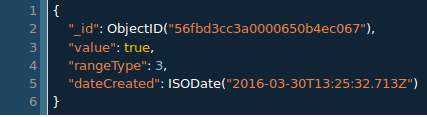
\includegraphics[width=\textwidth,natwidth=610,natheight=642]{Figures/DataStructures/RangesBoolean.png}
\caption{Documento dei Ranges Booleani}
\end{figure}


\begin{figure}[ht]
\centering
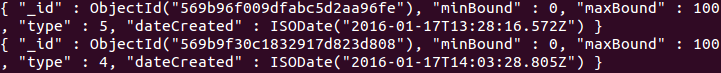
\includegraphics[width=\textwidth,natwidth=610,natheight=642]{Figures/DataStructures/RangesValues.png}
\caption{Documento dei Ranges di Valori}
\end{figure}

Si vuole far notare come sia comunque sempre presente un attributo di tipo data in modo da poter filtrare i range in base al tempo di inserimento e la presenza di un valore numerico che in questo caso rappresenta il tipo di range.

Per indicare il tipo di range si riporta il listato scala che indica tale tipologia.

\begin{figure}[ht]
\centering
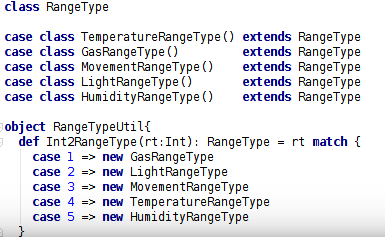
\includegraphics[scale=0.5,natwidth=610,natheight=642]{Figures/DataStructures/Ranges.png}
\caption{Valore numerico dei Ranges}
\end{figure}

\begin{center}
  \textbf{Collertion Sensors}
\end{center}

Per quanto riguarda la collezione dei sensori si utilizza un'apposita collection. Questa non sar\'a modificata spesso, e serve principalmente per eventuali evoluzioni del progetto, in modo che sia gi\'a presente. Anch'essi sono dotati di di tipo come i range e, per questa implementazione, i tipi coincidono. A livello di progetto per\'o si \'e deciso di mantenerli separati nel caso in un futuro questi divergano. Inseriamo di seguito un'immagine che rappresenta come \'e strutturato un documento di un sensore.

\begin{figure}[ht]
\centering
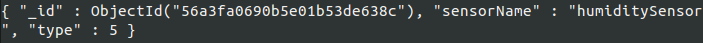
\includegraphics[scale=0.5,natwidth=610,natheight=642]{Figures/DataStructures/Sensors.png}
\caption{Rappresentazione a DB dei Sensori}
\end{figure}

\begin{center}
\textbf{Collection Data}
\end{center}

Per quanto riguarda la rappresentazione dei dati raccolti, anche in questo caso sono presenti 2 tipologie di dati:
\begin{itemize}
\item Dati Corretti: cio\'e quella tipologia di dati che rientrano all'interno del range prestabilito per la loro tipologia.
\item Dati Incorretti: quelli che invece non rientrano nella tipologia corretta e quindi vanno a violare il range attivo.
\end{itemize}

Come si pu\'o osservare il primo tipo \'e pi\'u semplice e ingloba i precedenti. Di seguito come fatto in precedenza si indica un esempio di struttura di un dato corretto e non corretto.

\begin{figure}[ht]
\centering
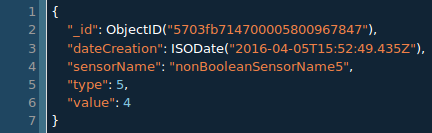
\includegraphics[scale=0.5,natwidth=610,natheight=642]{Figures/DataStructures/DataNoViolation.png}
\caption{Dato Corretto salvato in database}
\end{figure}

Come si pu\'o osservare \'e stato comunque inserito un valore per la violazione a \textit{null} in modo da poter distinguere meglio i dati violati da quelli invece corretti.

\begin{figure}[ht]
\centering
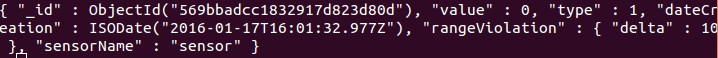
\includegraphics[scale=0.5,natwidth=610,natheight=642]{Figures/DataStructures/DataViolation.png}
\caption{Dato Non Corretto salvato in database}
\end{figure}

In questo caso appunto il valore della violazione non e' piu' nullo ma contiene un semplice campo \textit{delta} che indicher\'a la differenza rispetto al range. In particolare questo sar\'a positivo se il valore registrato supera il range attuale, negativo se invece \'e troppo basso o booleano se il tipo di sensoristica e quindi anche di range \'e booleano.

\begin{center}
  \textbf{Rappresentazione Dati Attraverso la Rete}
\end{center}

Oltre alla rappresentazione dei dati per quanto riguarda i dati salvati all'interno del Database \'e stato necessario concordare una rappresentazione di dati che verranno inviati attraverso la rete. Non necessariamente le due rappresentazioni devono coincidere in quanto, i dispositivi dai quali si ricavano i dati posso avere diversi formati e modalit\'a di ottenere tali valori, quindi di conseguenza questa rappresentazione \'e sbilanciata rispetto a chi invia i dati, cio\'e il sistema embedded.

Anche per la rappresentazione dei dati si \'e scelta la rappresentazione JSON in quanto questa \'e una delle pi\'u utilizzate nella comunicazione eterogenea via rete, si pone quindi come formato interoperabile tra varie tecnologie, come accade nel nostro caso.

Di seguito si riporta un esempio di dati in formato JSON:

\begin{lstlisting}[language=json]
  {
    "sensorName": "nomeSensore",
    "sensorType": 1,
    "value": true,
    "date": "2012-04-23T18:25:43.511Z"
  }
\end{lstlisting}

Si veda il tipo di sensore dai valori indicati precedentemente e si sottolinea che il tipo del campo \textit{value} pu\'o essere sia booleano che numerico.

\subsection{Introduzione All'Architettura di Progetto}

Nelle prossime sezioni si vuole inserire le modifiche che sono state fatte alla architettura logica appena introdotta, ma cercando di evitare di ripetere aspetti che non sono effettivamnete cambiati. Di conseguenza si \'e deciso di riportare solamente quegli aspetti che sono stati modificati in base alle scelte tecnologiche effettivamente fatte.\\
In ogni caso si \'e deciso di cercare il pi\'u possibile di sfruttare quanto gi\'a \'e stato concordato dagli analisti cercando di effettuare meno modifiche possibili all'architettura.

\begin{center}
  \textbf{Server}
\end{center}

\subsection{Struttura}

Vista l'introduzione della tecnologia in questa fase si \'e deciso di apportare alcune modifiche architetturali. Si riporta una lista di modifiche apportate all'architettura:

\begin{itemize}
  \item \textit{DataStructures:} Si \'e ritenuto necessario introdurre un'ulteriore package che non era stato previsto precedentemente contenente le rappresentazioni interne in forma di classi dei dati che circolano nel sistema, cos\'i come delle classi di utilit\'a che servono per la conversione, da e verso, questi dati.
  \item \textit{IDataFormatter:} Visto che le elaborazioni di trasformazione dei dati non richiedono tanta computazione si \'e deciso di eliminare il metodo che, dato un valore lo validava inglobandolo direttamente dentro il primo metodo che restituisce lo stream. Inoltre nella costruzione dello stream ci si \'e accorti che il valore dell'input non viene passato per parametro al metodo, ma viene gestito dall'infrastruttura, quindi si \'e deciso di eliminarlo. Spesso gli oggetti che validano e formattano i dati passano da una rappresentazione ad un'altra: tra valori JSON, BSON e classi interne per i dati.
  \item \textit{IDBDataFormatter:} Viene aggiunto un'ulteriore metodo che gestisce la creazione di dati da un formato inerente alle strutture dati presenti in un altro utilizzabile per lo storage dei dati nel DB. Questo metodo \'e estraneo a quelli per la costruzione di stream e serve per la gestione delle richieste di inserimento di un nuovo range.
  \item \textit{Eliminazione delle Factory:} Visto che la maggior parte delle classi che erano state pensate non inglobano uno stato, ma vengono utilizzate semplicemente per applicare delle computazioni allo stream allora sono state eliminate la maggior parte delle factory class. Grazie anche alla tecnologia scelta (scala) molte delle classi sono state convertite in objects (build-in singletons).
  \item \textit{Eliminazione della classe Configurator:} Si \'e deciso di eliminare tale classe in quando non \'e pi\'u possibile pensare a un entry point per l'applicazione, ma questa viene risvegliata attraverso chiamate rest e di conseguenza molti dei processi legati alla creazione di oggetti \'e stata ridotta.
\end{itemize}

\subsection{Interazione}

In questa parte si riporta la tecnologia che si \'e utilizzata per effettuare l'interazione che si \'e analizzata e indicata in fase di analisi, lo stream. In particolare si \'e notato che, il framework play\cite{PlayFramework} gi\'a gestisce attraverso delle sue strutture la possibilit\'a di operare attraverso stream di dati. Questa possibilit\'a \'e stata introdotta dal framework per gestire meglio dati parziali o casi che richiederebbero molto tempo, come ad esempio un'upload di file cospiquo. Nonostante tutto per\'o questo rientra nelle nostre necessit\'a e quindi ci avvarremo di questa astrazione per risolvere il nostro problema. Si riporta in bibliografia quindi la documentazione del framework che spiega il funzionamento di \textit{Enumerators,Iteratees e Enumeratees.} \cite{PlayStreaming}

Un'ulteriore modifica che va apportata visto che ci si trova in ambito web e si dispone di questo framework \'e la necessit\'a di eliminare alcune entit\'a previste precedentemente perch\'e, in fase realizzativa sono risultate ridondanti, ad esempio:
\begin{itemize}
\item \textbf{NewRangeDataReceiver:} Viene rimpiazzato dal controller che gestisce direttamente le richieste POST al sistema per la gestione dei dati provenienti dai form HTTP. Sar\'a questo componente, chiamato \textit{RangeEntryPoint} a validare direttamente i dati in arrivo e a chiamare poi gli elementi successivi nel flusso di dati per il salvataggio di un nuovo range. Si veda l'analisi del problema.
\end{itemize}

\subsection{Comportamento}

\begin{center}
  \textbf{Sistema Embedded}
\end{center}

\subsection{Struttura}
\subsection{Interazione}
\subsection{Comportamento}


\section{Implementazione}
\labelsec{Implementazione}
%===========================================================================

In questa fase bisognerebbe riportare il codice che implementa le varie parti, per\`o, per non appesantire troppo questa relazione che vuole essere una spiegazione alle scelte progettuali e di anali effettuate, si rimanda al lettore la revisione del codice. Di seguito si inserisce il link al repository contenente tutti i sorgenti del progetto stesso, nonch\`e il sorgente di tale documentazione.

\url{https://github.com/benkio/DomoticRoom}


\section{Testing}
\labelsec{Testing}
%===========================================================================

\subsection{Server}

Per quanto riguarda la parte di testing del server si sono implementati e impostati per lo sviluppo alcuni test unitari dell'applicativo. Il codice si pu\`o visionare all'interno dell'apposita cartella di test.

Particolare attenzione si \`e poi posta per i test di integrazione incui si \`e sviluppato un semplice script in fsharp che consente di simulare l'invio di dati dai valori random, strutturati come indicato nella sezione del progetto, all'endpoint specifico del server che si occupa di ricevere e salvare correttamente i dati. Questo ha consentito di parallelizzare al meglio il lavoro tra i membri del gruppo inquanto \`e possibile testare l'applicativo senza dover ottenere dei dati reali e conseguentemente impostare tutta l'infrastruttura ed inoltre ha impostato uno standard da seguire per l'invio dei dati verso il server che i client devono seguire affinch\'e non si verifichino problemi. Anche questo script \`e presente nel repository con le relative dipendenze.


\section{Deployment}
\labelsec{Deployment}
%===========================================================================

\section{Maintenance}
\labelsec{Maintenance}
%===========================================================================

%%% \begin{itemize}
%%% \item Titolo di studio:\\ \\
%%% \item Interessi particolari:\\ \\
%%% \item Ha sostenuto fino ad oggi il seguente numero di esami:\\ \\
%%% \item Deve ancora sostenere i seguenti esami del I anno:\\ \\
%%% \item Prevede di svolgere un tirocinio presso:\\ \\
%%% \item Prevede di laurearsi nella sessione:\\ \\
%%% \item Intende proseguire gli studi per conseguire: \\  \\  \\
%%%   	presso la sede universitaria di: \\ \\
%%% \item Intende entrare subito nel mondo del lavoro presso : \\ \\
%%% \end{itemize}

 
\appendix


\bibliographystyle{abbrv}
\bibliography{biblio}

\end{document}
